%%%%%%%%%%%%%%%%%%%%%%%%%%%%%%%%%%%%%%%%%%%%%%%%%%%%%%%%%%%%%%%%%%%%%%%%%%%%%%%%%
%%%%%%%%%%%%%%%%%%%%%%%%%%%%%%%%%%%%%%%%%%%%%%%%%%%%%%%%%%%%%%%%%%%%%%%%%%%%%%%%%
%%%%%%%%%%%%%%%%%%%%%%%%%%%%%%%%%%%%%%%%%%%%%%%%%%%%%%%%%%%%%%%%%%%%%%%%%%%%%%%%%
%%% TODO

% Define timing



%%%%%%%%%%%%%%%%%%%%%%%%%%%%%%%%%%%%%%%%%%%%%%%%%%%%%%%%%%%%%%%%%%%%%%%%%%%%%%%%%
%%%%%%%%%%%%%%%%%%%%%%%%%%%%%%%%%%%%%%%%%%%%%%%%%%%%%%%%%%%%%%%%%%%%%%%%%%%%%%%%%
%%%%%%%%%%%%%%%%%%%%%%%%%%%%%%%%%%%%%%%%%%%%%%%%%%%%%%%%%%%%%%%%%%%%%%%%%%%%%%%%%
%%% packages

\usepackage[english]{babel}
\usepackage{amsmath, amssymb}
\usepackage{array} 
\usepackage{tikz}
\usetikzlibrary{backgrounds}
%\usepackage{slashbox}
%\usepackage{pict2e}
%\usetikzlibrary{backgrounds}
%\usetikzlibrary{matrix}
\usepackage{url}
\usepackage{hyperref}
\usepackage{colordvi}
%\usepackage{xcolor, colortbl}
\usepackage{enumerate}
\usepackage[round]{natbib}
\usepackage{ifthen}
\usepackage{rotating}
\usepackage{varwidth}
\usetikzlibrary{arrows,automata,fit,calc,positioning,shapes,shapes.multipart} %



%%%%%%%%%%%%%%%%%%%%%%%%%%%%%%%%%%%%%%%%%%%%%%%%%%%%%%%%%%%%%%%%%%%%%%%%%%%%%%%%%
%%%%%%%%%%%%%%%%%%%%%%%%%%%%%%%%%%%%%%%%%%%%%%%%%%%%%%%%%%%%%%%%%%%%%%%%%%%%%%%%%
%%%%%%%%%%%%%%%%%%%%%%%%%%%%%%%%%%%%%%%%%%%%%%%%%%%%%%%%%%%%%%%%%%%%%%%%%%%%%%%%%
%%% beamer settings

\usetheme{Frankfurt}

\useoutertheme[subsection=false]{smoothbars}
\useinnertheme[shadow=true]{rounded}

\usecolortheme{orchid}
\usecolortheme{whale}

\setbeamertemplate{navigation symbols}{}

\setbeamertemplate{footline}[text line]{\color{dkgreen} \bf
  \insertshortauthor \hfill \insertshorttitle \hfill 15th Reasoning
  Web Summer School (RW
  2019) \hfill \insertframenumber/\inserttotalframenumber}

\setbeamersize{text margin left=0.5cm} 
\setbeamersize{text margin right=0.5cm} 



%%%%%%%%%%%%%%%%%%%%%%%%%%%%%%%%%%%%%%%%%%%%%%%%%%%%%%%%%%%%%%%%%%%%%%%%%%%%%%%%%
%%%%%%%%%%%%%%%%%%%%%%%%%%%%%%%%%%%%%%%%%%%%%%%%%%%%%%%%%%%%%%%%%%%%%%%%%%%%%%%%%
%%%%%%%%%%%%%%%%%%%%%%%%%%%%%%%%%%%%%%%%%%%%%%%%%%%%%%%%%%%%%%%%%%%%%%%%%%%%%%%%%
%%% commands

%%%%%%%%%%%%%%%%%%%%%%%%%%%%%%%%%%%%%%%%%%%%%%%%%%%%%%%%%%%%%%%%%%%%%%%%%%%%%%%%%
%%%%%%%%%%%%%%%%%%%%%%%%%%%%%%%%%%%%%%%%%%%%%%%%%%%%%%%%%%%%%%%%%%%%%%%%%%%%%%%%%
%%%%%%%%%%%%%%%%%%%%%%%%%%%%%%%%%%%%%%%%%%%%%%%%%%%%%%%%%%%%%%%%%%%%%%%%%%%%%%%%%
%%% slides stuff

\newcommand{\blocknode}[5]{\node (#1) at #2 {%
    \begin{minipage}{3.5cm}\begin{block}{#4}
        \begin{overlayarea}{3.5cm}{#3}
        #5\end{overlayarea}\end{block}\end{minipage}};}
\newcommand{\smallblocknode}[5]{\node (#1) at #2 {%
    \begin{minipage}{3.0cm}\begin{block}{#4} \begin{overlayarea}{3.0cm}{#3}
    #5\end{overlayarea}\end{block}\end{minipage}};}
\newcommand{\redsmallblocknode}[5]{\node (#1) at #2 {%
    \begin{minipage}{3.0cm}\begin{alertblock}{#4} \begin{overlayarea}{3.0cm}{#3}
    #5\end{overlayarea}\end{alertblock}\end{minipage}};}



\renewcommand{\newblock}{}
\definecolor{ToDoColor}{rgb}{0,0.16,0.90} %blue
\definecolor{OutlineColor}{rgb}{0.2,0.8,0.2} %green
\definecolor{CommentColor}{rgb}{0.90,0.16,0} %red
\definecolor{dkgreen}{rgb}{0,0.5,0}
\definecolor{mLightBrown}{rgb}{0.71,0.40,0.11}
\definecolor{mLightGreen}{rgb}{0.56,0.93,0.56}
\newcommand<>{\textblue}[1]{{\color#2{blue}#1}}
\newcommand<>{\textred}[1]{{\color#2{red}#1}}
\newcommand<>{\textgreen}[1]{{\color#2{green}#1}}
\newcommand<>{\textdkgreen}[1]{{\color#2{dkgreen}#1}}
\newcommand<>{\textorange}[1]{{\color#2{orange}#1}}
\newcommand<>{\textyellow}[1]{{\color#2{yellow}#1}}

\newcommand{\ie}{i.\,e.}
\newcommand{\eg}{e.\,g.}
\newcommand{\cf}{cf.}

\newcommand{\notesym}{\ensuremath{\to}} 
\newcommand{\noteblk}[1]{
\begin{block}{}
#1
\end{block}} 

\newcommand{\lectureslides}[1]{\ifthenelse{\value{VERSION}=0}{#1}{}}
\newcommand{\nolectureslides}[1]{\ifthenelse{\not\value{VERSION}=0}{#1}{}}
\newcommand{\posthandout}[1]{\ifthenelse{\value{VERSION}=1}{#1}{}}
\newcommand{\noposthandout}[1]{\ifthenelse{\not\value{VERSION}=1}{#1}{}}
\newcommand{\prehandout}[1]{\ifthenelse{\value{VERSION}=2}{#1}{}}
\newcommand{\noprehandout}[1]{\ifthenelse{\not\value{VERSION}=2}{#1}{}}


\newcommand{\images}{../IMAGES}
\graphicspath{{../IMAGES/}}
\newcommand{\rovergoal}[1]{
\includegraphics[scale=0.06]{rovergoal#1.png}
}


%%%%%%%%%%%%%%%%%%%%%%%%%%%%%%%%%%%%%%%%%%%
%%% defs, propositions, etc

\newenvironment{mydef}[1]{

\begin{block}{#1}
}{
\end{block}
}

\newenvironment{myprop}[1]{

\begin{block}{Proposition (#1)}
}{
\end{block}
}

\newenvironment{myproof}{

\begin{block}{Proof}
}{
\end{block}
}



%%%%%%%%%%%%%%%%%%%%%
%%%
%%% quiz: highlight ``correct'' (green, 2), ``discuss''
%%% (orange, 1), ``false'' (red, 0) in post-handouts only!

\newcommand{\quiz}[9]{

\prehandout{
\begin{block}{Quiz}
\textbf{#1}
\vspace{-0.15cm}
\begin{columns}
\begin{column}{.45\textwidth}
\begin{itemize}
\item[\textblue{(A):}] #2\vspace{-0.05cm}
\item[\textblue{(C):}] #4
\end{itemize}
\end{column}
\begin{column}{.45\textwidth}
\begin{itemize}
\item[\textblue{(B):}] #3\vspace{-0.05cm}
\item[\textblue{(D):}] #5
\end{itemize}
\end{column}
\end{columns}
\end{block}
}

\lectureslides{
\begin{block}{Quiz}
\textbf{#1}
\vspace{-0.15cm}
\begin{columns}
\begin{column}{.45\textwidth}
\begin{itemize}
\item[\textblue{(A):}] #2\vspace{-0.05cm}
\item[\textblue{(C):}] #4
\end{itemize}
\end{column}
\begin{column}{.45\textwidth}
\begin{itemize}
\item[\textblue{(B):}] #3\vspace{-0.05cm}
\item[\textblue{(D):}] #5
\end{itemize}
\end{column}
\end{columns}
\end{block}
}

\posthandout{
\begin{block}{Quiz}
\textbf{#1}
\vspace{-0.15cm}
\begin{columns}
\begin{column}{.45\textwidth}
\begin{itemize}
\item[\textblue{(A):}] \ifthenelse{#6=0}{\textred{#2}}{\ifthenelse{#6=1}{\textorange{#2}}{\ifthenelse{#6=2}{\textdkgreen{#2}}{}}}\vspace{-0.05cm}
\item[\textblue{(C):}] \ifthenelse{#8=0}{\textred{#4}}{\ifthenelse{#8=1}{\textorange{#4}}{\ifthenelse{#8=2}{\textdkgreen{#4}}{}}}
\end{itemize}
\end{column}
\begin{column}{.45\textwidth}
\begin{itemize}
\item[\textblue{(B):}] \ifthenelse{#7=0}{\textred{#3}}{\ifthenelse{#7=1}{\textorange{#3}}{\ifthenelse{#7=2}{\textdkgreen{#3}}{}}}\vspace{-0.05cm}
\item[\textblue{(D):}] \ifthenelse{#9=0}{\textred{#5}}{\ifthenelse{#9=1}{\textorange{#5}}{\ifthenelse{#9=2}{\textdkgreen{#5}}{}}}
\end{itemize}
\end{column}
\end{columns}
\end{block}
}

}




%%%%%%%%%%%%%%%%%%%%%
%%%
%%% quiztwo: highlight ``correct'' (green, 2), ``discuss''
%%% (orange, 1), ``false'' (red, 0) in post-handouts only!

\newcommand{\quiztwo}[5]{

\prehandout{
\begin{block}{Quiz}
\textbf{#1}
\vspace{-0.15cm}
\begin{columns}
\begin{column}{.45\textwidth}
\begin{itemize}
\item[\textblue{(A):}] #2
\end{itemize}
\end{column}
\begin{column}{.45\textwidth}
\begin{itemize}
\item[\textblue{(B):}] #3
\end{itemize}
\end{column}
\end{columns}
\end{block}
}

\lectureslides{
\begin{block}{Quiz}
\textbf{#1}
\vspace{-0.15cm}
\begin{columns}
\begin{column}{.45\textwidth}
\begin{itemize}
\item[\textblue{(A):}] #2
\end{itemize}
\end{column}
\begin{column}{.45\textwidth}
\begin{itemize}
\item[\textblue{(B):}] #3
\end{itemize}
\end{column}
\end{columns}
\end{block}
}

\posthandout{
\begin{block}{Quiz}
\textbf{#1}
\vspace{-0.15cm}
\begin{columns}
\begin{column}{.45\textwidth}
\begin{itemize}
\item[\textblue{(A):}] \ifthenelse{#4=0}{\textred{#2}}{\ifthenelse{#4=1}{\textorange{#2}}{\ifthenelse{#4=2}{\textdkgreen{#2}}{}}}
\end{itemize}
\end{column}
\begin{column}{.45\textwidth}
\begin{itemize}
\item[\textblue{(B):}] \ifthenelse{#5=0}{\textred{#3}}{\ifthenelse{#5=1}{\textorange{#3}}{\ifthenelse{#5=2}{\textdkgreen{#3}}{}}}
\end{itemize}
\end{column}
\end{columns}
\end{block}
}

}




%%%%%%%%%%%%%%%%%%%%%%%%%%%%%%%%%%%%%%%%%%%%%%%%%%%%%%%%%%%%%%%%%%%%%%%%%%%%%%%%%
%%%%%%%%%%%%%%%%%%%%%%%%%%%%%%%%%%%%%%%%%%%%%%%%%%%%%%%%%%%%%%%%%%%%%%%%%%%%%%%%%
%%%%%%%%%%%%%%%%%%%%%%%%%%%%%%%%%%%%%%%%%%%%%%%%%%%%%%%%%%%%%%%%%%%%%%%%%%%%%%%%%
%%% commands from paper

\newcommand{\defined}[1]{\textblue{#1}}


%%%%%%%%%%% heuristics %%%%%%%%%%%%

\newcommand{\hrefine}{\ensuremath{h_{r}}}
\newcommand{\hboth}{\ensuremath{h_{r+b}}}
\newcommand{\hbellman}{\ensuremath{h_{b}}}

\newcommand{\abs}{\mathcal{A}}
\newcommand{\numtasks}[1]{\tiny{(#1)}}

%\newcommand{\formalspacesave}{}

\newcommand{\naturals}{\ensuremath{\mathbb N}}
\newcommand{\reals}{{\mathbb{R}}}
\newcommand{\powerset}{{\mathcal{P}}}

\newcommand{\tuple}[1]{\ensuremath{\langle #1 \rangle}}

\newcommand{\astar}{\ensuremath{\textrm{A}^*}}

\newcommand{\poly}{\textbf{P}}
\newcommand{\np}{\textbf{NP}}
\newcommand{\pspace}{\textbf{PSPACE}}


%%%%%%%%%%%%%%%%%%%%%%%%%%%%%%
%%%%% Generic Framework
\newcommand{\task}{\ensuremath{\tau}}
%\newcommand{\task}{\ensuremath{\cal T}}
\newcommand{\plan}{\ensuremath{\pi}}
\newcommand{\plans}{\ensuremath{\Pi}}
%\newcommand{\alltasks}{\ensuremath{\cal T}}
\newcommand{\allplans}{\ensuremath{\cal P}}
\newcommand{\true}{\ensuremath{\mathit{true}}}
\newcommand{\false}{\ensuremath{\mathit{false}}}

\newcommand{\prop}{\ensuremath{p}}
\newcommand{\propq}{\ensuremath{q}}
\newcommand{\props}{\ensuremath{P}}
\newcommand{\propsatom}{\ensuremath{{P^{\text{\textup{A}}}}}}
\newcommand{\propscomp}{\ensuremath{{P^{\text{\textup{C}}}}}}

\newcommand{\modelsof}[2]{\ensuremath{{\cal M}_#1(#2)}}
\newcommand{\entails}[3]{\ensuremath{#1 \models #2 \Rightarrow #3}}
\newcommand{\notentails}[3]{\ensuremath{#1 \not\models #2 \Rightarrow #3}}
\renewcommand{\iff}[3]{\ensuremath{#1 \models #2 \Leftrightarrow #3}}
\renewcommand{\equiv}[2]{\ensuremath{[#2]_{#1}}}
%
%% \renewcommand{\implies}[1]{\ensuremath{\Rightarrow_{#1}}}
%% \renewcommand{\iff}[1]{\ensuremath{\Leftrightarrow_{#1}}}
%% \renewcommand{\equiv}[2]{\ensuremath{[#1]_{#2}}}

\newcommand{\pdo}[1]{\ensuremath{\Rightarrow_{#1}}}
\newcommand{\pda}[1]{\ensuremath{\Phi_{#1}}}

\newcommand{\entailsuff}{\ensuremath{\Rightarrow_{\mathit{suff}}}}

\newcommand{\deps}{\ensuremath{D}}


%%%%%%%%%%%%%%%%%%%%%%%%%%%%%%
%%%%% Planning Tasks

\newcommand{\vars}{\ensuremath{V}}
\newcommand{\acts}{\ensuremath{A}}
\newcommand{\init}{\ensuremath{I}}
\newcommand{\goal}{\ensuremath{G}}
\newcommand{\goalhard}{\ensuremath{G^{\text{\textup{hard}}}}}
\newcommand{\goalsoft}{\ensuremath{G^{\text{\textup{soft}}}}}
\newcommand{\cost}{{\ensuremath{c}}}
\newcommand{\pre}{\ensuremath{\mathit{pre}}}
\newcommand{\eff}{\ensuremath{\mathit{eff}}}

\newcommand{\variables}[1]{\ensuremath{{\cal V}(#1)}}
\newcommand{\apply}[1]{\ensuremath{[[#1]]}}

\newcommand{\costbound}{{\ensuremath{b}}}


%%%%%%%%%%%%%%%%%%%%%%%%%%%%%%
%%%%% Goal facts

\newcommand{\goalpropsatom}{\ensuremath{{P^{\text{\textup{GA}}}}}}
\newcommand{\goalpropscomp}{\ensuremath{{P^{\text{\textup{GC}}}}}}

\newcommand{\geprops}{\ensuremath{{P^{\text{\textup{GE}}}}}}
\newcommand{\gedeps}{\ensuremath{{D^{\text{\textup{GE}}}}}}

\newcommand{\dgeprops}{\ensuremath{{P^{\text{\textup{DGE}}}}}}
\newcommand{\dgedeps}{\ensuremath{{D^{\text{\textup{DGE}}}}}}



%%%%%%%%%%%%%%%%%%%%%%%%%%%%%%
%%%%% Heuristic Functions

\newcommand{\hstar}{\ensuremath{h^*}}
\newcommand{\hplus}{\ensuremath{h^+}}

\newcommand{\hone}{\ensuremath{h^1}}
\newcommand{\htwo}{\ensuremath{h^2}}
\newcommand{\hm}{\ensuremath{h^m}}
\newcommand{\hc}{\ensuremath{h^C}}
\newcommand{\hcx}{\ensuremath{h^{C \cup X}}}
\newcommand{\uc}{\ensuremath{u^C}}
\newcommand{\ucx}{\ensuremath{u^{C \cup X}}}
\newcommand{\hmax}{\ensuremath{h^{\text{\textup{max}}}}}
\newcommand{\hff}{\ensuremath{h^{\text{\textup{FF}}}}}
\newcommand{\hlmcut}{\ensuremath{h^{\text{\textup{LM-cut}}}}}
\newcommand{\hms}{\ensuremath{h^{\text{M\&S}}}}


%%%%%%%%%%%%%%%%%%%%%%%%%%%%%%
%%%%% Stackelberg notation

\newcommand{\leader}{\ensuremath{L}}
\newcommand{\follower}{\ensuremath{F}}

\newcommand{\bestresponse}{\ensuremath{{BR}}}

\newcommand{\actsL}{\ensuremath{\acts^{\leader}}}
\newcommand{\actsF}{\ensuremath{\acts^{\follower}}}
\newcommand{\goalF}{\goal^{\follower}}

\newcommand{\statesL}{\ensuremath{\states^{\leader}}}

\newcommand{\equilibrium}{\ensuremath{\states^*}}

\newcommand{\strategyL}{\ensuremath{\strategy^{\leader}}}
\newcommand{\strategyF}{\ensuremath{\strategy^{\follower}}}

\newcommand{\strategystarL}{\ensuremath{\strategy^{\leader*}}}
\newcommand{\strategystarF}{\ensuremath{\strategy^{\follower*}}}

\newcommand{\costL}{\ensuremath{\leader}}
\newcommand{\costF}{\ensuremath{\follower}}
\newcommand{\coststarL}{\ensuremath{\leader^*}}
\newcommand{\coststarF}{\ensuremath{\follower^*}}
\newcommand{\costapproxL}{\ensuremath{\leader^+}}
\newcommand{\costapproxF}{\ensuremath{\follower^+}}

\newcommand{\hstackel}{\ensuremath{h^{\text{\textup{Stackel}}}}}
\newcommand{\Hstackel}{\ensuremath{H}}
\newcommand{\upperF}{\ensuremath{\mathsf{up}^{\follower}}}
\newcommand{\lowerL}{\ensuremath{\mathsf{low}^{\leader}}}
\newcommand{\upperL}{\ensuremath{\mathsf{up}^{\leader}}}

%%%%%%%%%%%%%%%%%%%%%%%%%%%%%%
%%%%% Search algorithms

\newcommand{\result}{\ensuremath{\hat{S}}}

\newcommand{\open}{\ensuremath{\mathsf{Open}}}
\newcommand{\closed}{\ensuremath{\mathsf{Explored}}}
\newcommand{\comment}[1]{{\color{red} /* #1 */}}

\newcommand{\searchalg}{\ensuremath{\textup{leader-follower-search}}}

\newcommand{\bounds}{\ensuremath{\mathbb{B}}}

%%% Planning domains
\newcommand{\airport}               {{Airport}}
\newcommand{\barman }               {{Barman}}
\newcommand{\blocksworld}           {{Blocksworld}}
\newcommand{\childsnack}           {{Childsnack}}
\newcommand{\depots}                {{Depots}}
\newcommand{\driverlog}             {{Driverlog}}
\newcommand{\elevators}             {{Elevators}}
\newcommand{\floortile}             {{Floortile}}
\newcommand{\freecell}              {{FreeCell}}
\newcommand{\grid}                  {{Grid}}
\newcommand{\gripper}               {{Gripper}}
\newcommand{\hiking}               {{Hiking}}
\newcommand{\logistics}             {{Logistics}}
\newcommand{\simplelogistics}       {{Simple-Logistics}}
\newcommand{\movie}                 {{Movie}}
\newcommand{\extmovie}              {{Ext-Movie}}
\newcommand{\promela}               {{Promela}}
\newcommand{\diningphilosophers}    {{Dining-Philosophers}}
\newcommand{\opticaltelegraph}      {{Optical-Telegraph}}
\newcommand{\miconic}               {{Miconic}}
\newcommand{\mystery}               {{Mystery}}
\newcommand{\mprime}                {{Mprime}}
\newcommand{\nomystery}             {{Nomystery}}
\newcommand{\openstacks}            {{Openstacks}}
\newcommand{\parcprinter}           {{Parcprinter}}
\newcommand{\parking}               {{Parking}}
\newcommand{\pathways}              {{Pathways}}
\newcommand{\pegsol}                {{Pegsol}}
\newcommand{\pipesworld}            {{Pipesworld}}
\newcommand{\pipesworldnotankage}   {{Pipesworld-NoTankage}}
\newcommand{\pipesworldtankage}     {{Pipesworld-Tankage}}
\newcommand{\pipesworldnotankageshort}   {{Pipes-NoTank}}
\newcommand{\pipesworldtankageshort}     {{Pipes-Tank}}
\newcommand{\psr}                   {{PSR}}
\newcommand{\rovers}                {{Rovers}}
\newcommand{\satellite}             {{Satellite}}
\newcommand{\scanalyzer}            {{Scanalyzer}}
\newcommand{\schedule}              {{Schedule}}
\newcommand{\schedulestrips}        {{Schedule-Strips}}
\newcommand{\seqschedule}           {{SeqSchedule}}
\newcommand{\sokoban}               {{Sokoban}}
\newcommand{\storage}               {{Storage}}
\newcommand{\tetris}               {{Tetris}}
\newcommand{\thoughtful}               {{Thoughtful}}
\newcommand{\tidybot}               {{Tidybot}}
\newcommand{\tpp}                   {{TPP}}
\newcommand{\trucks}                {{Trucks}}
\newcommand{\transport}             {{Transport}}
\newcommand{\woodworking}           {{Woodworking}}
\newcommand{\woodworkingshort}      {{Woodwork}}
\newcommand{\visitall}              {{Visitall}}
\newcommand{\zenotravel}            {{Zenotravel}}

\newcommand{\airportveryshort}{Airport}
\newcommand{\barmanveryshort}{Barman}
\newcommand{\blocksworldveryshort}{Blocksworld}
\newcommand{\childsnackveryshort}           {{Childsnack}}
\newcommand{\depotsveryshort}{Depots}
\newcommand{\driverlogveryshort}{Driverlog}
\newcommand{\elevatorsveryshort}{Elevators}
\newcommand{\floortileveryshort}{Floortile}
\newcommand{\freecellveryshort}{Freecell}
\newcommand{\gripperveryshort}{Gripper}
\newcommand{\gridveryshort}{Grid}
\newcommand{\hikingveryshort}               {{Hiking}}
\newcommand{\logisticsveryshort}{Logistics}
\newcommand{\miconicveryshort}{Miconic}
\newcommand{\mprimeveryshort}{Mprime}
\newcommand{\mysteryveryshort}{Mystery}
\newcommand{\nomysteryveryshort}{NoMystery}
\newcommand{\openstacksveryshort}{Openstacks}
\newcommand{\parkingveryshort}{Parking}
\newcommand{\parcprinterveryshort}{Parcprinter}
\newcommand{\pathwaysveryshort}{Pathways}
\newcommand{\pegsolveryshort}{Pegsol}
\newcommand{\pipesworldnotankageveryshort}   {{PipesNoTank}}
\newcommand{\pipesworldtankageveryshort}     {{PipesTank}}
\newcommand{\psrveryshort}{PSR}
\newcommand{\roversveryshort}{Rovers}
\newcommand{\satelliteveryshort}{Satellite}
\newcommand{\scanalyzerveryshort}{Scanalyzer}
\newcommand{\sokobanveryshort}{Sokoban}
\newcommand{\storageveryshort}               {{Storage}}
\newcommand{\tetrisveryshort}               {{Tetris}}
\newcommand{\thoughtfulveryshort}       {{Thoughtful}}
\newcommand{\tidybotveryshort}{Tidybot}
\newcommand{\tppveryshort}{TPP}
\newcommand{\transportveryshort}{Transport}
\newcommand{\trucksveryshort}{Trucks}
\newcommand{\visitallveryshort}{Visitall}
\newcommand{\woodworkingveryshort}{Woodworking}
\newcommand{\zenotravelveryshort}{Zenotravel}

\newcommand{\pentesting}{{Pentest}}
\newcommand{\pentestingshort}{{Pentest}}




















%%%%%%%%%%%%%%%%%%%%%%%%%%%%%%%%%%%%%%%%%%%%%%%%%%%%%%%%%%%%%%%%%%%%%%%%%%%%%%%%%
%%%%%%%%%%%%%%%%%%%%%%%%%%%%%%%%%%%%%%%%%%%%%%%%%%%%%%%%%%%%%%%%%%%%%%%%%%%%%%%%%
%%%%%%%%%%%%%%%%%%%%%%%%%%%%%%%%%%%%%%%%%%%%%%%%%%%%%%%%%%%%%%%%%%%%%%%%%%%%%%%%%
%%% Title Page & Agenda

\title[Explainable AI Planning]{Explainable AI Planning:\\ Overview and the Case of Contrastive Explanation}

\subtitle{Part 2: Explaining the Space of Plans}

\author[Hoffmann and Magazzeni]{J\"org Hoffmann and Daniele Magazzeni}

\institute[Saarland University and King's College London]{

\includegraphics[height=1.7cm]{saarland-university} \hspace{0.3cm} 
\includegraphics[height=1.7cm]{kcl} 
}

\date{September 23, 2019}


\AtBeginSection[]
{
  \begin{frame}<beamer>{Agenda}
    \tableofcontents[currentsection]
  \end{frame}
}

\begin{document}

\frame{\titlepage}

\begin{frame}{Agenda}
\tableofcontents
\end{frame}



%%%%%%%%%%%%%%%%%%%%%%%%%%%%%%%%%%%%%%%%%%%%%%%%%%%%%%%%%%%%%%%%%%%%%%%%%%%%%%%%%
%%%%%%%%%%%%%%%%%%%%%%%%%%%%%%%%%%%%%%%%%%%%%%%%%%%%%%%%%%%%%%%%%%%%%%%%%%%%%%%%%
%%%%%%%%%%%%%%%%%%%%%%%%%%%%%%%%%%%%%%%%%%%%%%%%%%%%%%%%%%%%%%%%%%%%%%%%%%%%%%%%%
%%% Introduction
%
%%% Timing: XX min

\section[Introduction]{Introduction}
\subsection*{}

\begin{frame}{The Traditional View of AI Planning}

\centering

\medskip

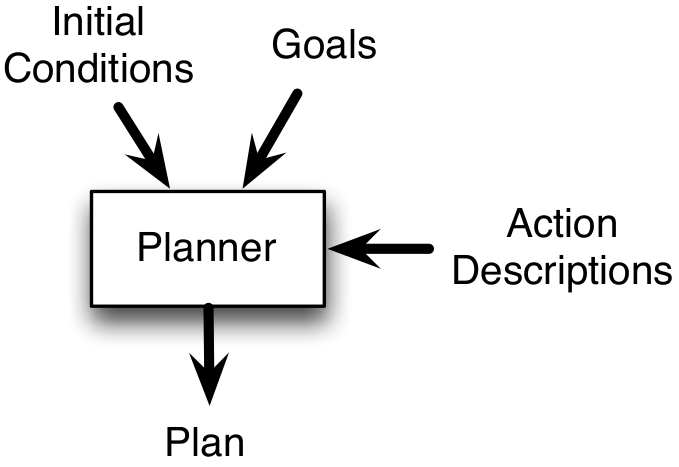
\includegraphics[height=0.5\textheight]{david-traditional}

\medskip

{\footnotesize (Figure from [\cite{smith:aaai-12}])}

\end{frame}


\begin{frame}{A Typical Reality: Interactive Decision Making}

\centering

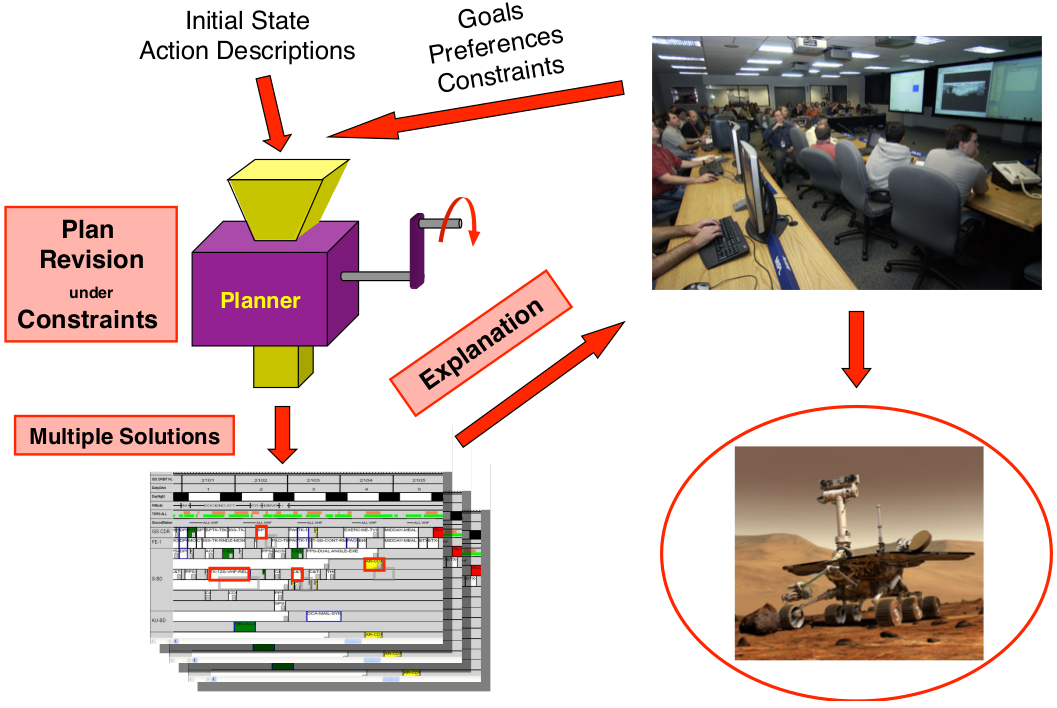
\includegraphics[height=0.75\textheight]{david-process}

\medskip

{\footnotesize (Figure from [\cite{smith:aaai-12}])}

\end{frame}


\begin{frame}{The Problem}

\centering

\begin{tikzpicture}
\node[] (human) at (-3,-2.3) {\huge Human};
\node[] (ai) at (2.8,-2.3) {\huge AI};

\visible<1|handout:0>{
\node[] (i1) at (0,0) {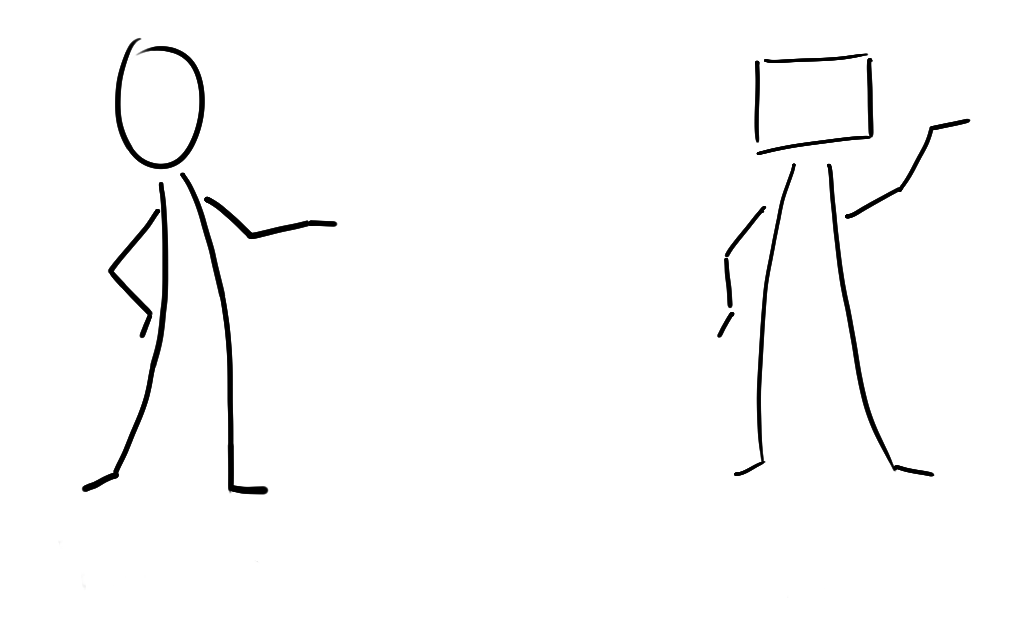
\includegraphics[scale=0.25]{part2-intro1.png}};
}

\visible<2|handout:0>{
\node[] (i2) at (-0.28,0.85) {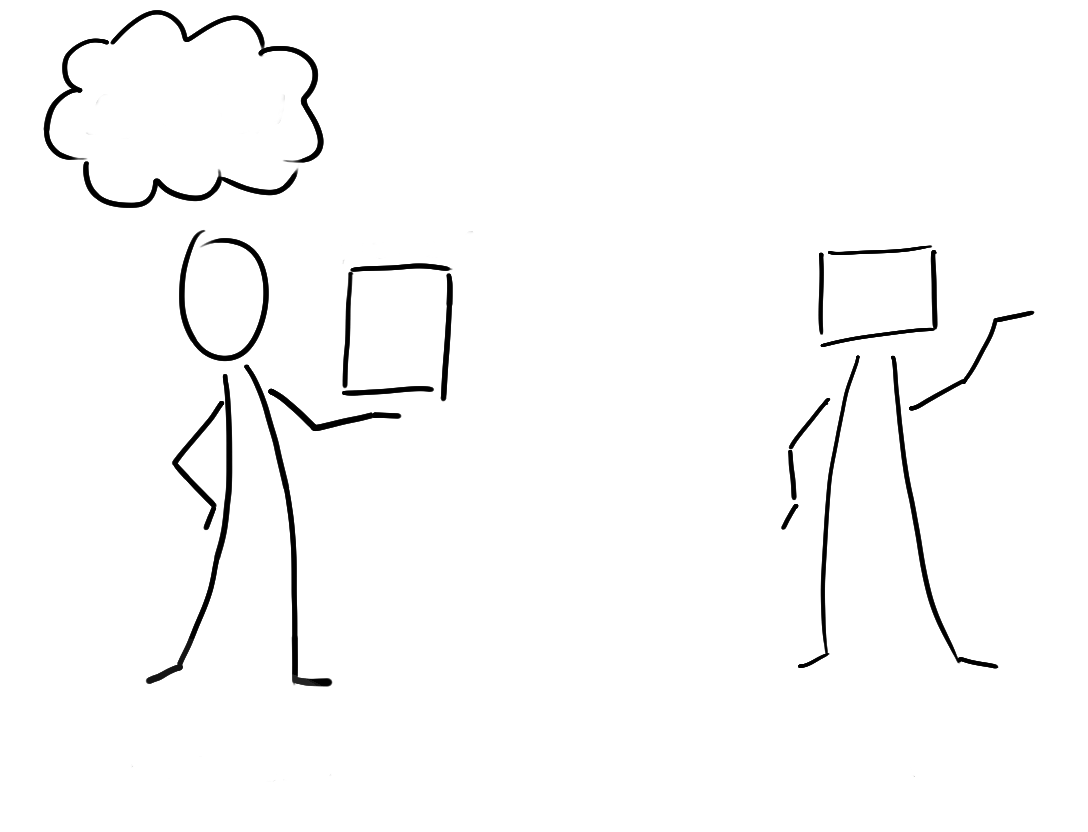
\includegraphics[scale=0.25]{part2-intro2.png}};
\node[] (solution) at (-3.3,3.5) {\large Solution};
\node[] (task) at (-1.6,2.5) {\large Task};
}

\visible<3|handout:0>{
\node[] (i3) at (0,0.85) {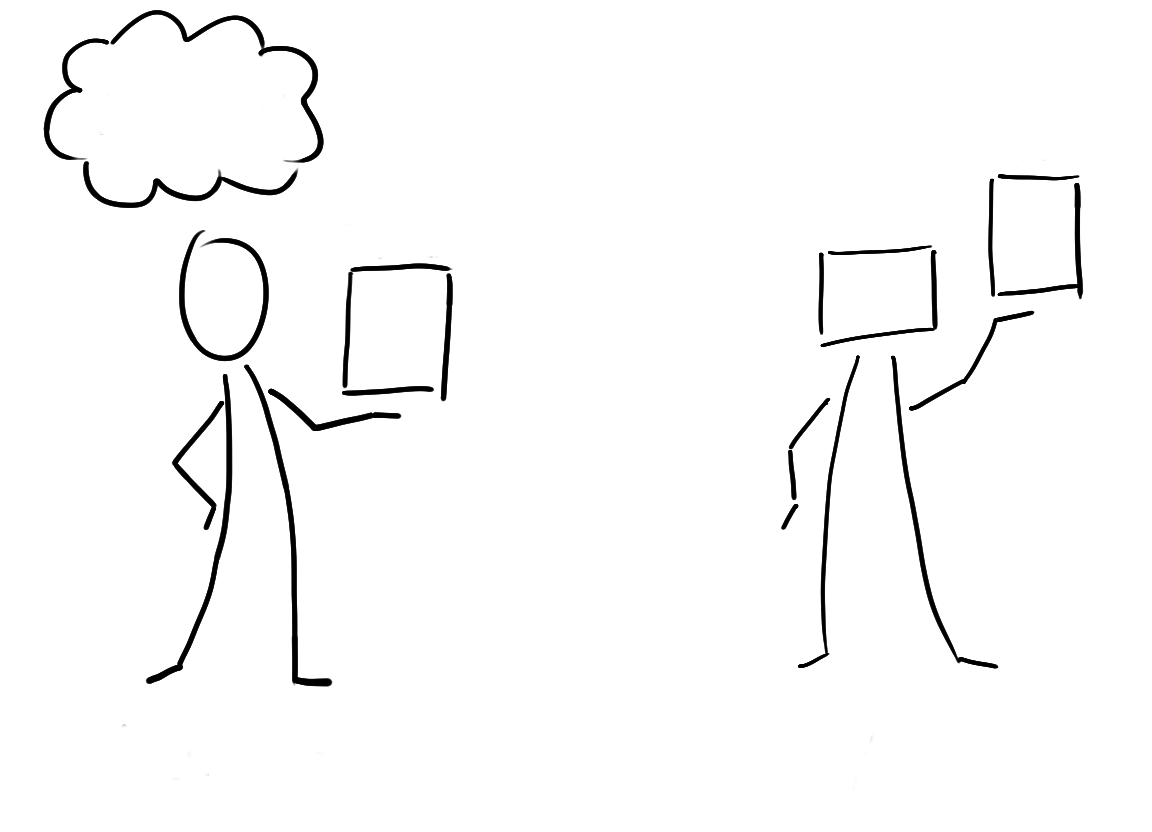
\includegraphics[scale=0.25]{part2-intro3.png}};
\node[] (solution) at (-3.3,3.5) {\large Solution};
\node[] (task) at (-1.6,2.5) {\large Task};
\node[] (plan) at (4.0,3.2) {\large Plan};
}

\visible<4|handout:0>{
\node[] (i4) at (0.28,0.57) {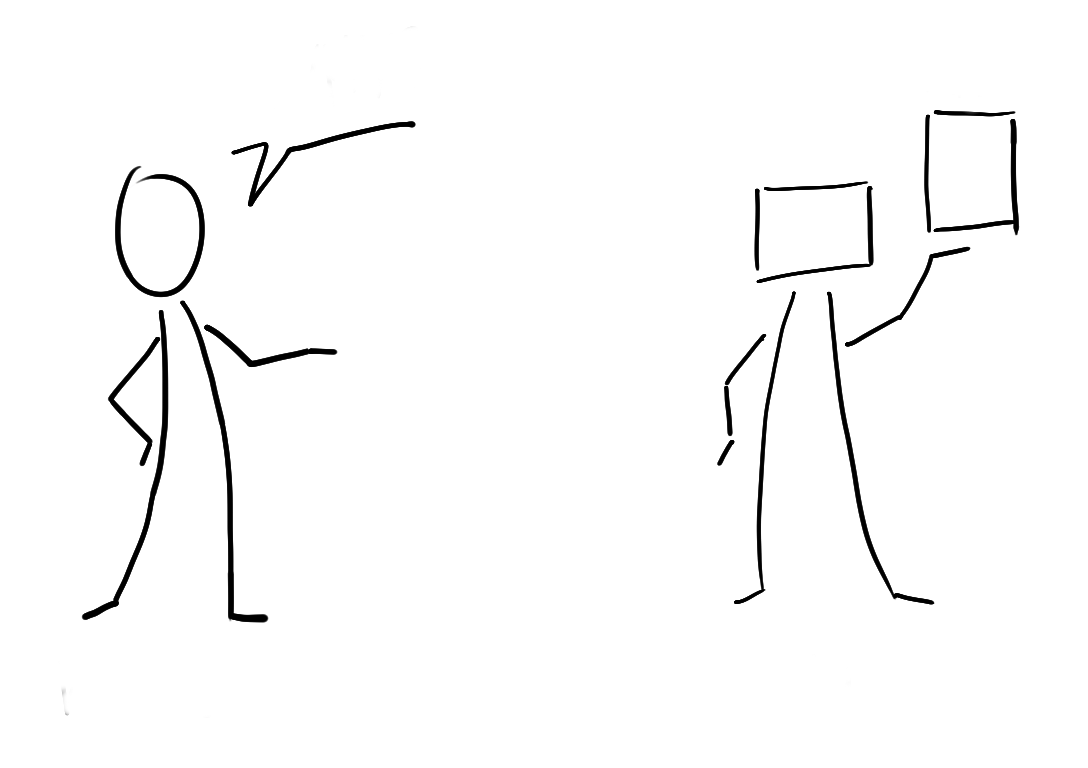
\includegraphics[scale=0.25]{part2-intro4.png}};
\node[align=center] (why) at (-2.0,3.4) {Why this plan and \\not another plan?};
\node[] (plan) at (4.0,3.2) {\large Plan};
}

\visible<5|handout:1>{
\node[] (i5) at (-0.285,0.29) {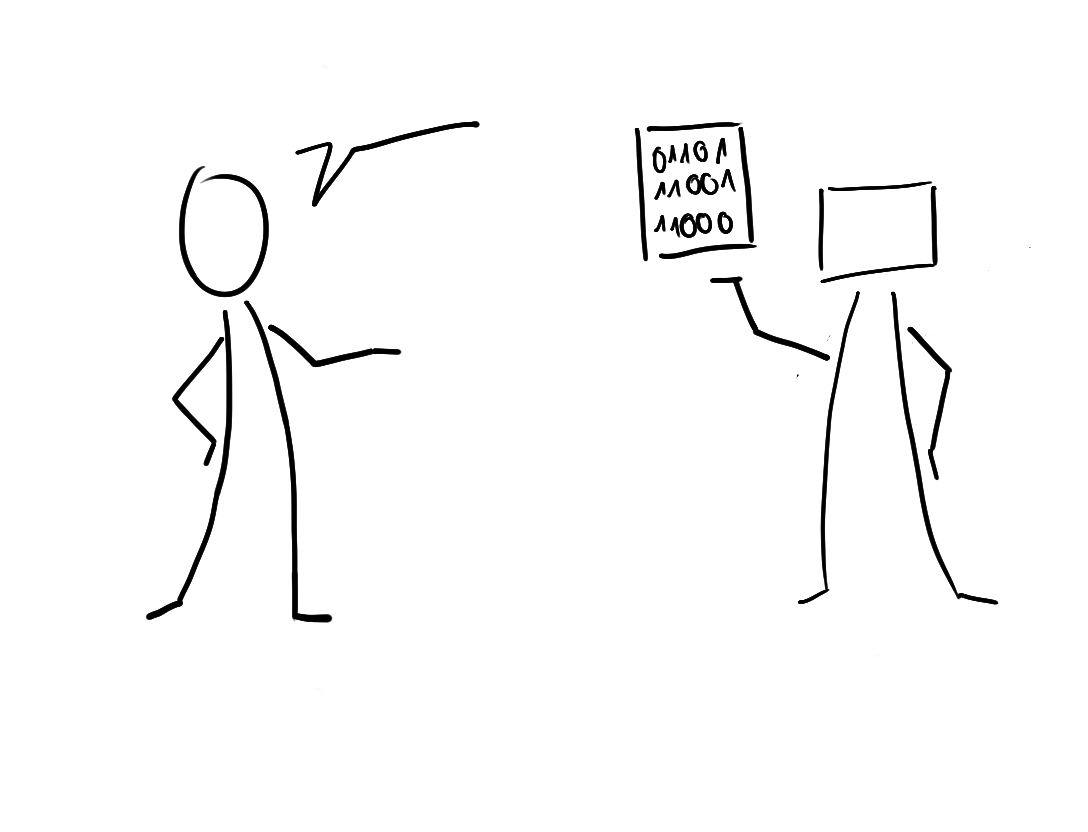
\includegraphics[scale=0.25]{part2-intro5.png}};
\node[align=center] (why) at (-2.0,3.4) {Why this plan and \\not another plan?};
}

\visible<6|handout:0>{
\node[] (i6) at (0,0.57) {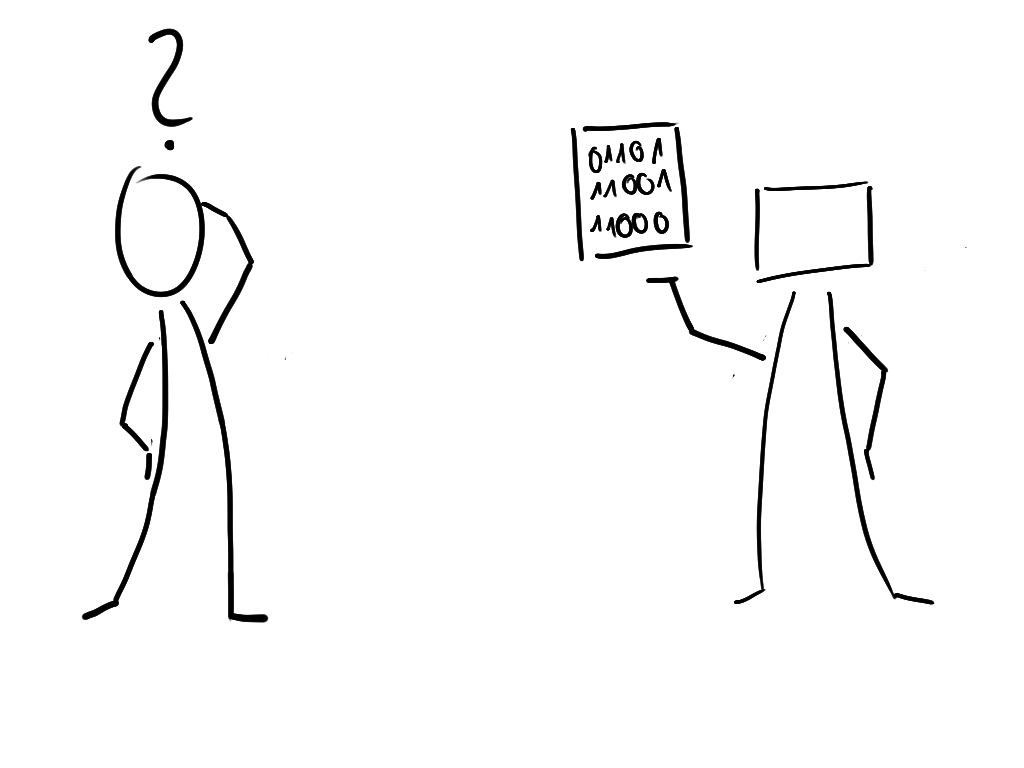
\includegraphics[scale=0.25]{part2-intro6.png}};
}
\end{tikzpicture}

\medskip

\end{frame}


\begin{frame}{Our Approach: Plan-Property Dependencies}

\centering

\begin{tikzpicture}
\node[] (human) at (-3,-2.3) {\huge Human};
\node[] (ai) at (2.8,-2.3) {\huge AI};

\visible<1|handout:0>{
\node[] (i3) at (0,0.85) {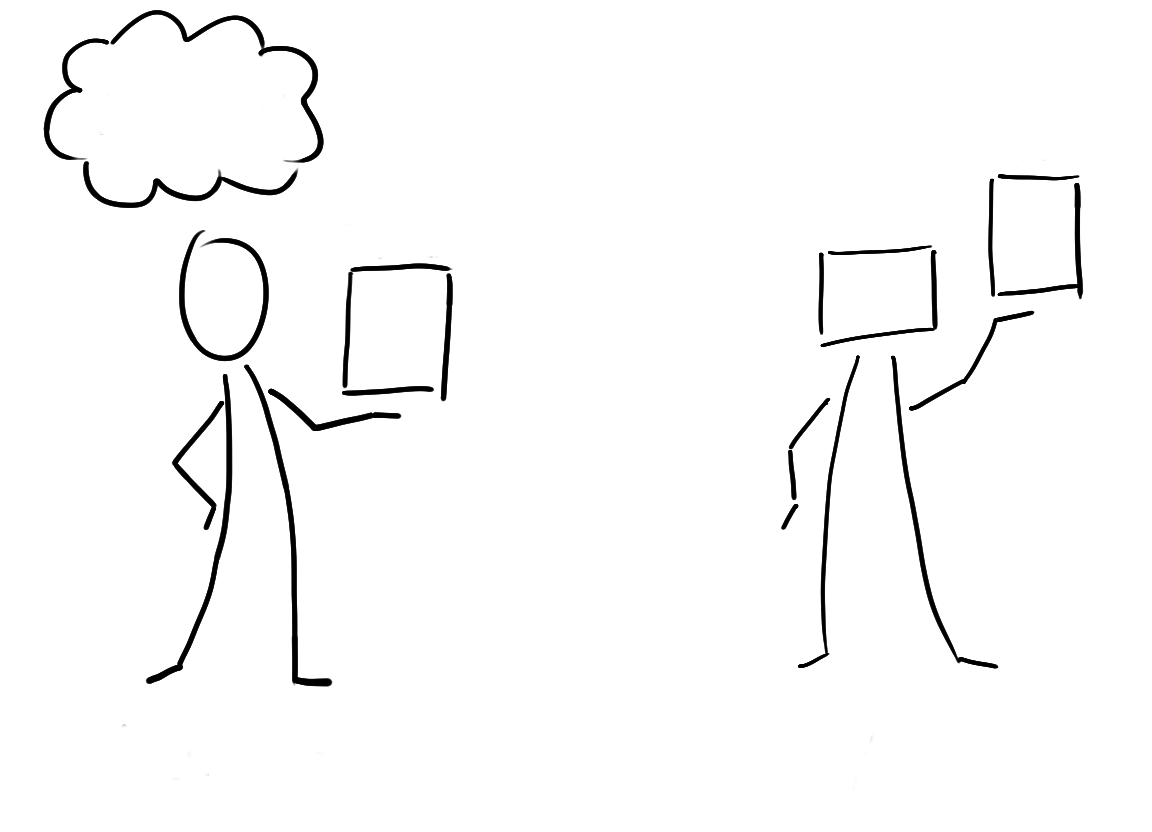
\includegraphics[scale=0.25]{part2-intro3.png}};
\node[] (solution) at (-3.3,3.5) {\large Solution};
\node[] (task) at (-1.6,2.5) {\large Task};
\node[] (plan) at (4.0,3.2) {\large Plan};
}

\visible<2|handout:0>{
\node[] (i4) at (0.28,0.57) {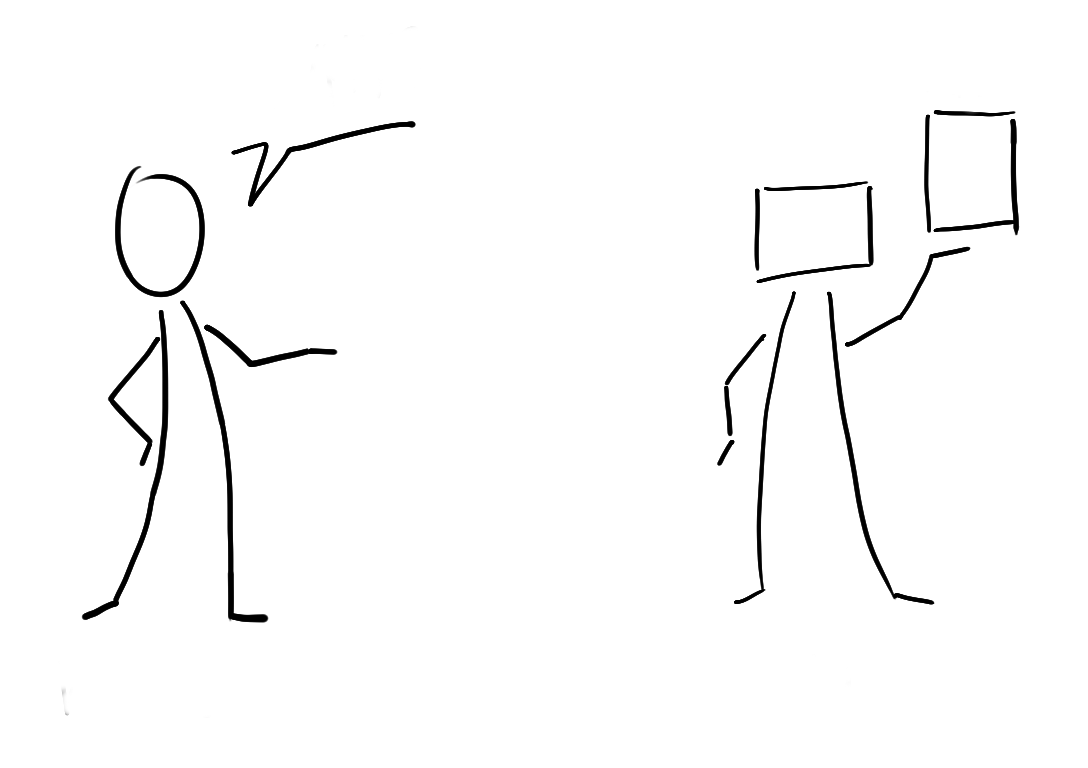
\includegraphics[scale=0.25]{part2-intro4.png}};
\node[align=center] (why) at (-2.0,3.4) {Why this plan and \\not another plan?};
\node[] (plan) at (4.0,3.2) {\large Plan};
}

\visible<3|handout:0>{
\node[] (i4) at (0.28,0.57) {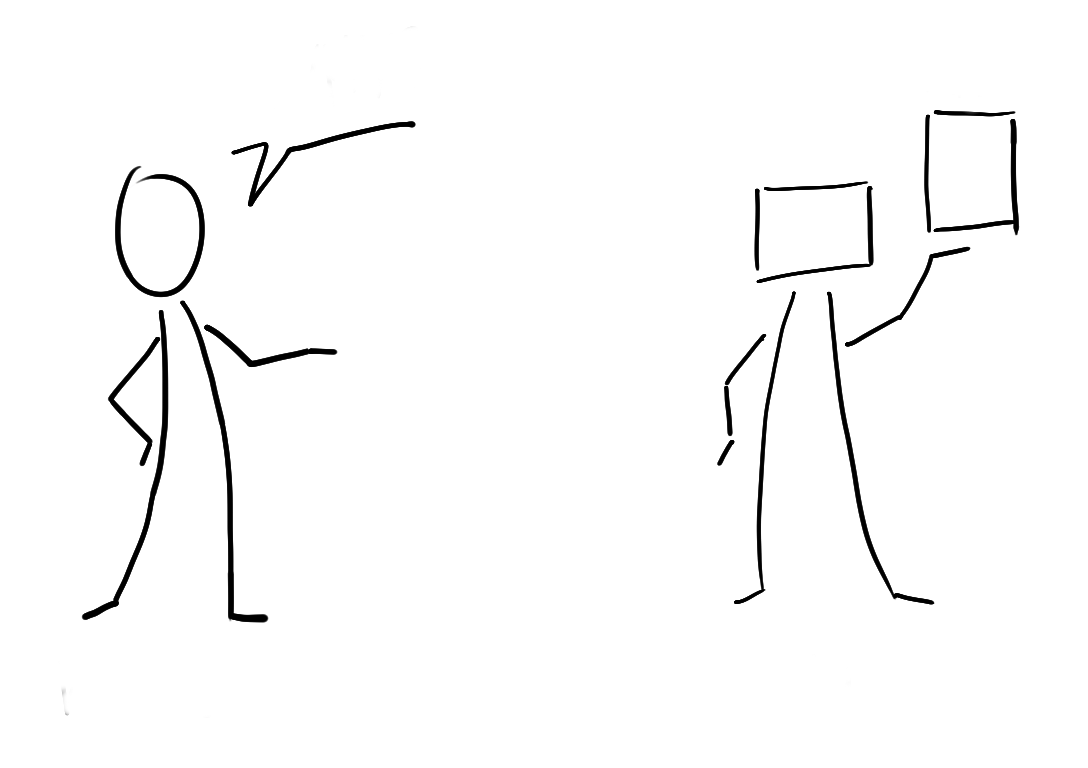
\includegraphics[scale=0.25]{part2-intro4.png}};
\node[align=center] (why) at (-2.0,3.4) {Why does this plan\\ not have \textcolor{dkgreen}{property A?}};
\node[] (plan) at (4.0,3.2) {\large Plan};
}

\visible<4|handout:1>{
\node[] (i5) at (-0.285,0.29) {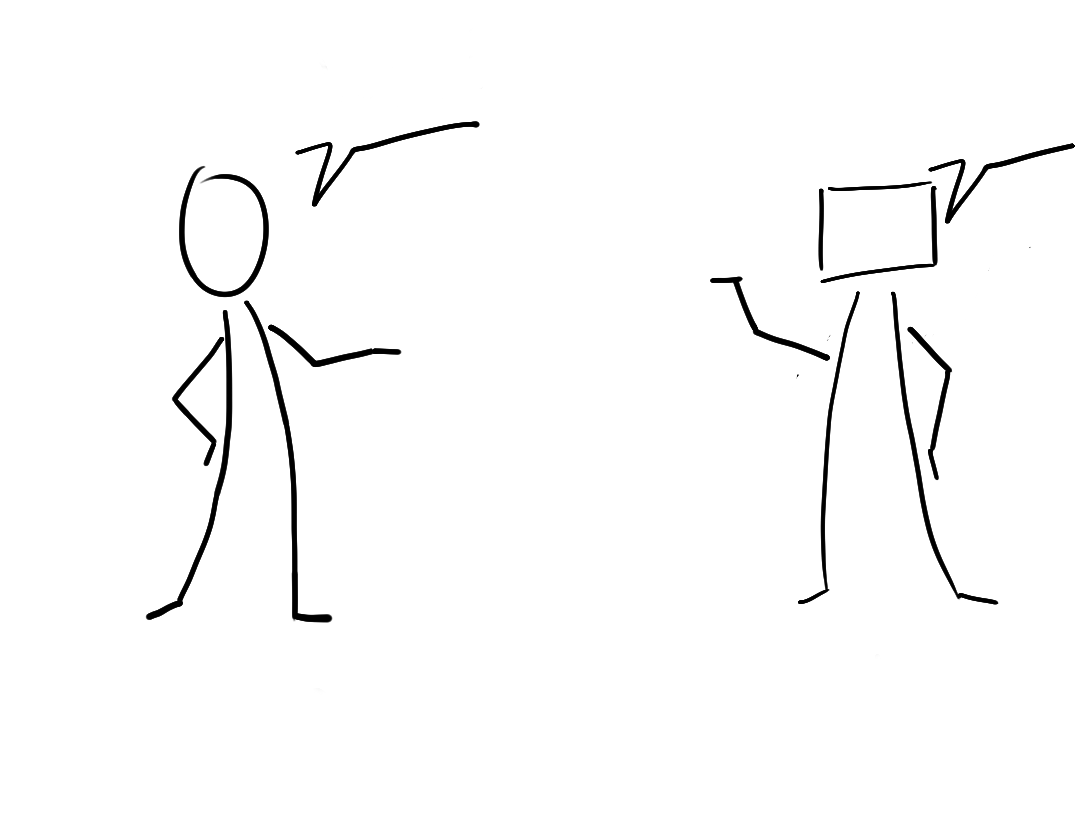
\includegraphics[scale=0.333]{part2-intro5b.png}};
\node[align=center] (why) at (-2.0,3.4) {Why does this plan\\ not have \textcolor{dkgreen}{property A?}};
\node[align=center] (dependency) at (3.5,3.4) {Because all plans\\ with \textcolor{dkgreen}{property A}\\ have \textcolor{red}{property B!}};
}

\visible<5|handout:0>{
\node[] (i6) at (0,0.57) {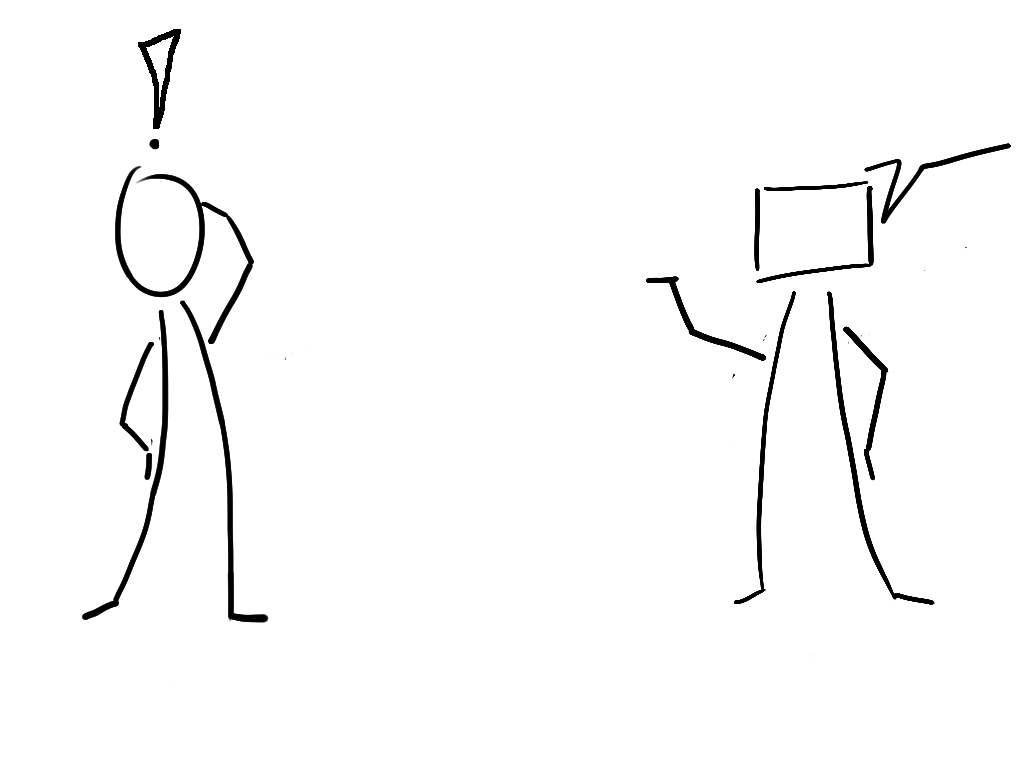
\includegraphics[scale=0.333]{part2-intro6b.png}};
\node[align=center] (dependency) at (3.5,3.4) {Because all plans\\ with \textcolor{dkgreen}{property A}\\ have \textcolor{red}{property B!}};
}
\end{tikzpicture}

\medskip

\end{frame}


\begin{frame}{Our Approach in Interactive AI Planning}

\centering

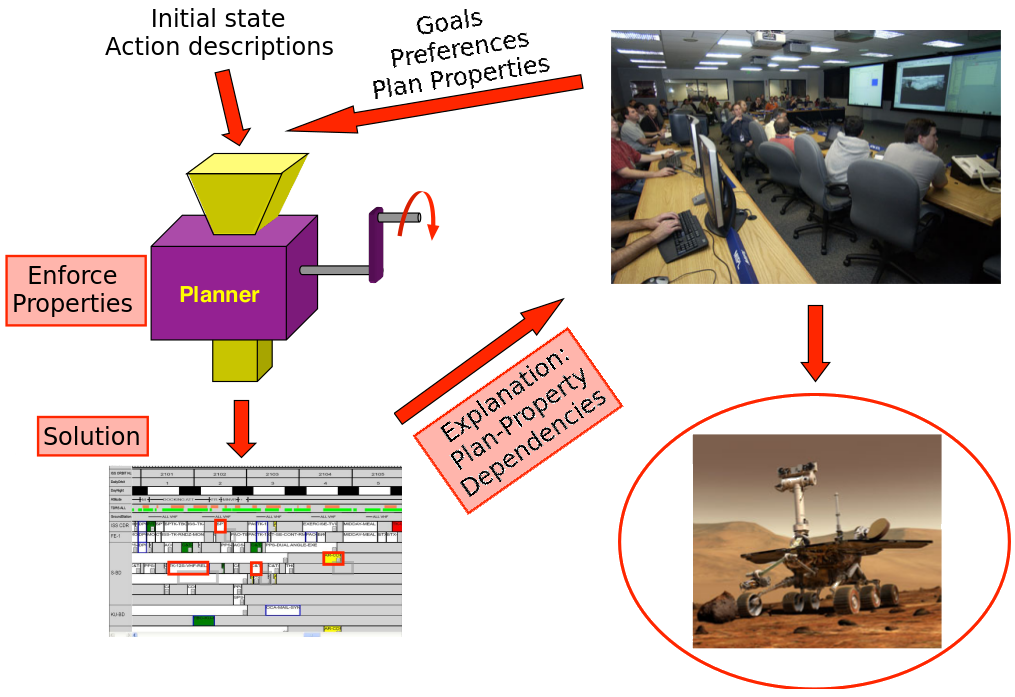
\includegraphics[height=0.75\textheight]{david-process-adapted}

\medskip

{\footnotesize (Figure adapted from [\cite{smith:aaai-12}])}

\end{frame}


\begin{frame}{(Toy) Example: IPC Rovers}

\centering

\vspace{-0.2cm}

\begin{tikzpicture}
\visible<1->{
\node[] (r1) at (1.5,2) {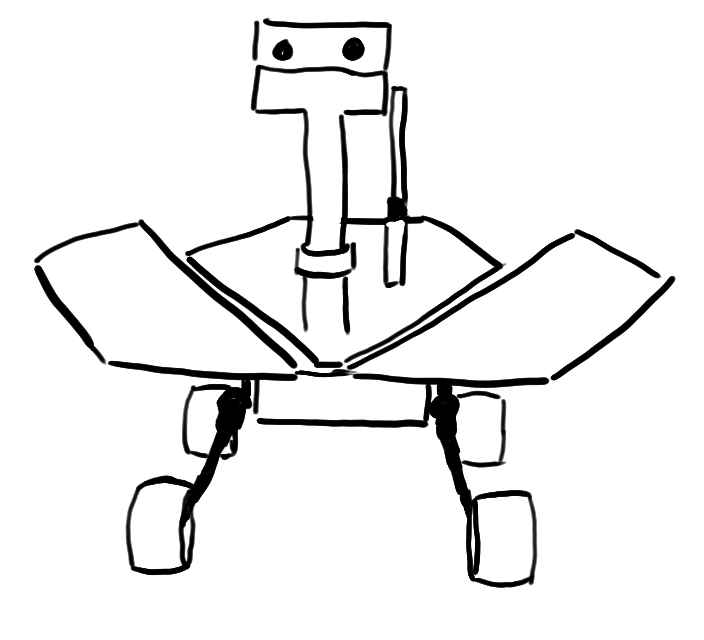
\includegraphics[scale=0.07]{rover2.png}};
\node[] (b1) at (0.5,2.5) {
\includegraphics[scale=0.07]{battery.png}};
\node[] (r2) at (-5,-2.5) {
\includegraphics[scale=0.07]{rover1.png}};
\node[] (b2) at (-5,-3.5) {
\includegraphics[scale=0.07]{battery.png}};

\node[] (m) at (0,0) {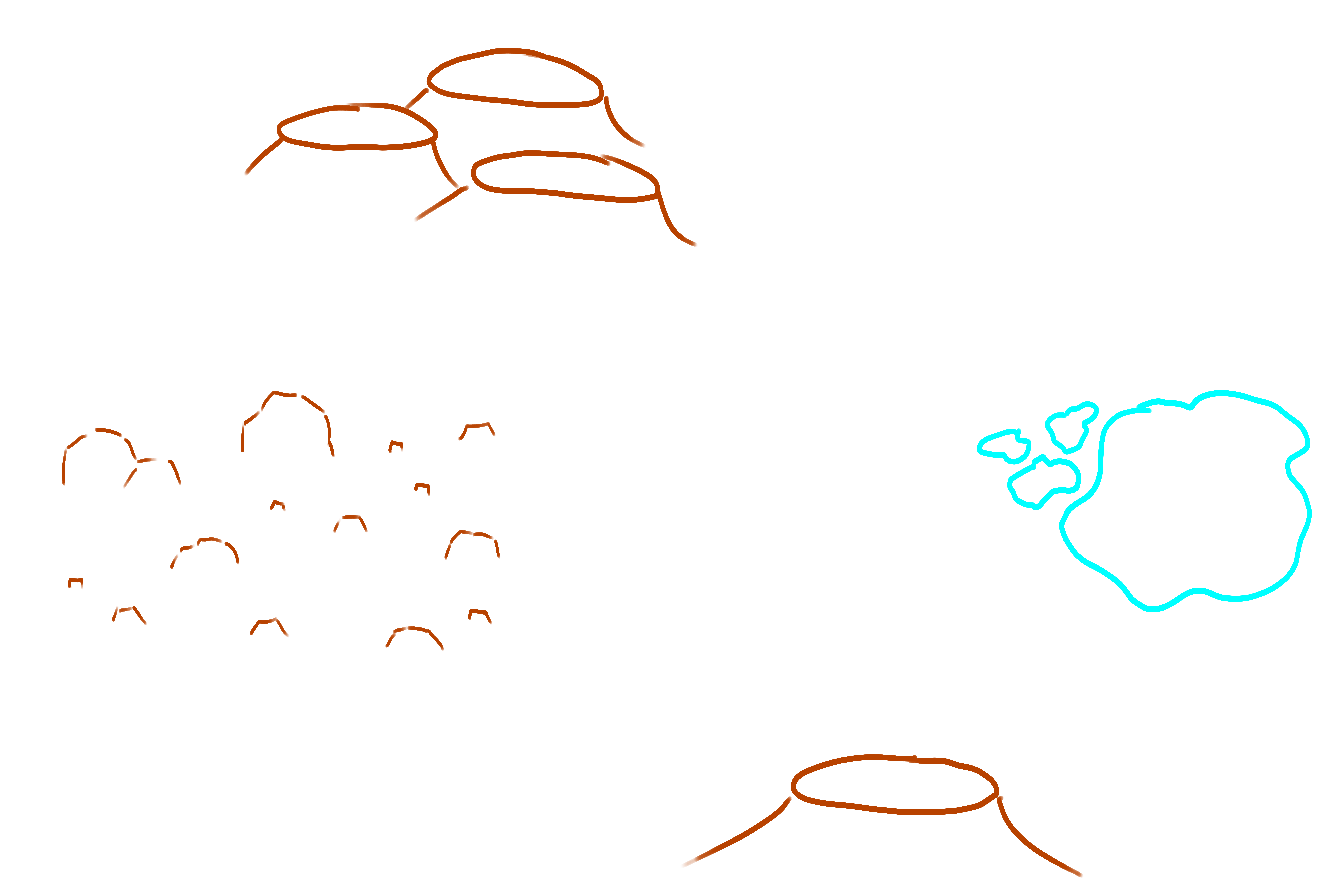
\includegraphics[scale=0.2]{mars.png}};
}

\visible<2->{
\node[] (g) at (-1.9,-4) {\Large \textbf{goal}:};
\node[] (i1) at (-0.5,-4) {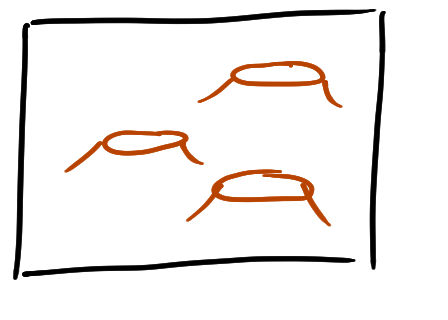
\includegraphics[scale=0.1]{rovergoal1.png}};
\node[] (i2) at (0.8,-4) {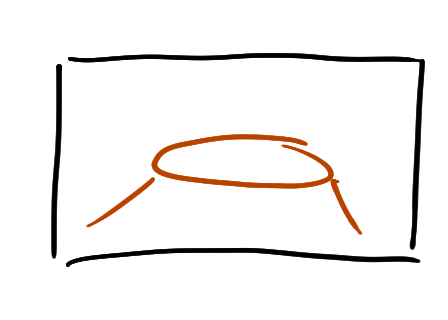
\includegraphics[scale=0.1]{rovergoal2.png}};
\node[] (i3) at (2.5,-4) {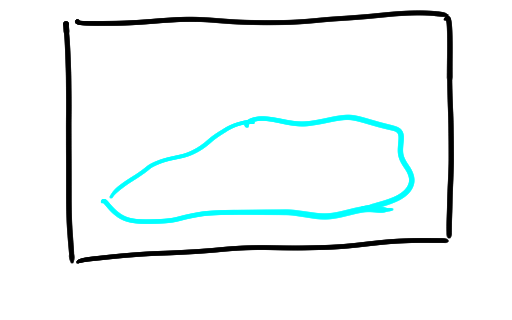
\includegraphics[scale=0.1]{rovergoal3.png}};
\node[] (i1) at (-0.5,-3.3) {$I_1$};
\node[] (i2) at (0.8,-3.4) {$I_2$};
\node[] (i3) at (2.5,-3.3) {$I_3$};
}

\visible<3->{
\node[draw, circle, inner sep=3pt] (l1) at (-3,-3) {$L_1$};
\node[draw, circle, inner sep=3pt] (l2) at (-2.1,1.3) {$L_2$};
\node[draw, circle, inner sep=3pt] (l3) at (-0.5,-1) {$L_3$};
\node[draw, circle, inner sep=3pt] (l4) at (3,2) {$L_4$};
\node[draw, circle, inner sep=3pt] (l5) at (1.8,0) {$L_5$};
\node[draw, circle, inner sep=3pt] (l6) at (3.2,-2.5) {$L_6$};

\draw[thick] (l1) to (l2);
\draw[thick] (l1) to (l3);
\draw[thick] (l2) to (l3);
\draw[thick] (l3) to (l5);
\draw[thick] (l4) to (l5);
\draw[thick] (l4) to (l6);
\draw[thick] (l5) to (l6);
}

\visible<4->{
\node[align=left] (actions) at (-5.5,2) {
%\Large \textbf{actions}:\\
%\vspace*{0.2cm}
\begin{varwidth}{4.0cm}
\begin{itemize}
\item $drive(R_i,L_x,L_y)$
\item $takeImage(I_x,R_y)$
\end{itemize}
\end{varwidth}
};
}
\end{tikzpicture}
	
\end{frame}



%%%%%%%%%%%%%%%%%%%%%%%%%%%%%%%%%%%%%%%%%%%%%%%%%%%%%%%%%%%%%%%%%%%%%%%%%%%%%%%%%
%%%%%%%%%%%%%%%%%%%%%%%%%%%%%%%%%%%%%%%%%%%%%%%%%%%%%%%%%%%%%%%%%%%%%%%%%%%%%%%%%
%%%%%%%%%%%%%%%%%%%%%%%%%%%%%%%%%%%%%%%%%%%%%%%%%%%%%%%%%%%%%%%%%%%%%%%%%%%%%%%%%
%%% Oversubscription Planning
%
%%% Timing: XX min

\section[OSP]{Oversubscription Planning}
\subsection*{}

\begin{frame}{Oversubscription Planning}

\begin{mydef}{Oversubscription Planning \hfill {\footnotesize [\cite{smith:icaps-04,domshlak:mirkis:jair-15}]}}
An \defined{OSP task} is a tuple \textred{$\task =
(\vars,\allowbreak\acts,\allowbreak\cost,\allowbreak\init,\allowbreak\goalhard,\allowbreak\goalsoft,\allowbreak\costbound)$}:
\begin{itemize}
\item \vars\ Variables, \acts\ Actions, \cost\ action-cost function, 
\init\ initial state;
\item \goalhard\ \defined{hard} goal;
\item \goalsoft\ \defined{soft} goal;
\item $\costbound \in \reals^+_0$ \defined{cost bound}.
\end{itemize}
As before: outcome state of applicable action sequence $\plan$ denoted
$s\apply{\plan}$. \plan\ is a \defined{plan} if
cost \textred{$\leq \costbound$ and
$\goalhard \subseteq \init\apply{\plan}$}.
%
%% An \defined{oversubscription planning (OSP) task} is a tuple $\task =
%% (\vars,\allowbreak\acts,\allowbreak\cost,\allowbreak\init,\allowbreak\goalhard,\allowbreak\goalsoft,\allowbreak\costbound)$
%% like an FDR task but with two goals -- the \defined{hard} goal
%% \goalhard\ and the \defined{soft} goal \goalsoft, assumed to be
%% defined on disjoint sets of variables -- as well as an additional
%% \defined{cost bound} $\costbound \in \reals^+_0$. A \defined{plan} is
%% an action sequence \plan\ whose summed-up cost is $\leq \costbound$
%% and where $\goalhard \subseteq \init\apply{\plan}$.
%
\end{mydef}

\bigskip \pause

\textbf{Plan quality:} Usually additive soft-goal rewards. \pause Here:

\begin{itemize}
\item User preferences hard to specify/elicitate. Iterative planning instead.
\item Goal-exclusion dependencies to support that process.
\end{itemize}

\medskip

\end{frame}


% NOTE: Talk flow better when pointing this out only on next slide:
% energy limited, plan achieves goals 1 and 3 but not goal 2.
%
%% \begin{frame}{Mars Rover OSP}

%% \centering

%% \begin{tikzpicture}
%% \node[] (el) at (0,0) {\Large energy limit};
%% \node[] (el) at (3,0) {
\includegraphics[scale=0.2]{battery-low.png}};
%% \end{tikzpicture}

%% \bigskip \medskip

%% \visible<2>{
%% \begin{tabular}{c|c|c}
%% 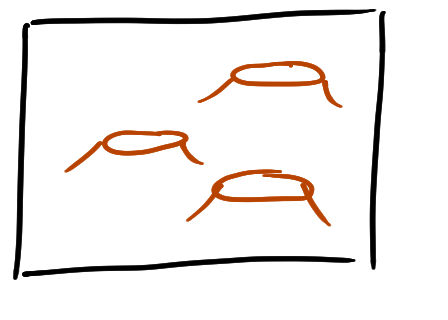
\includegraphics[scale=0.15]{rovergoal1.png} &
%% 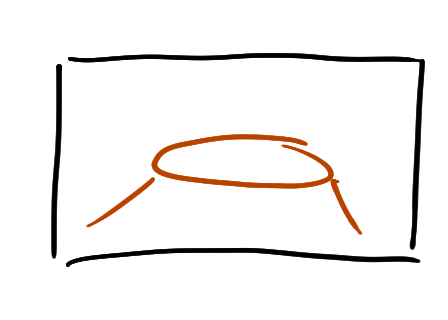
\includegraphics[scale=0.15]{rovergoal2.png} &
%% 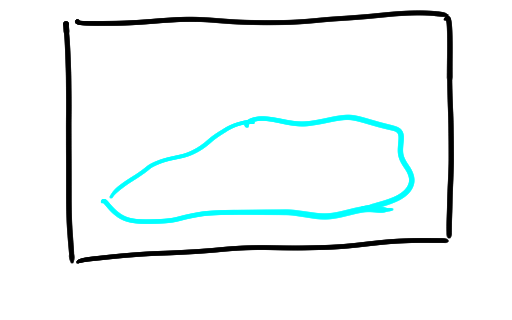
\includegraphics[scale=0.15]{rovergoal3.png} \\\hline

%% 
\includegraphics[scale=0.1]{yes.png} &
%% 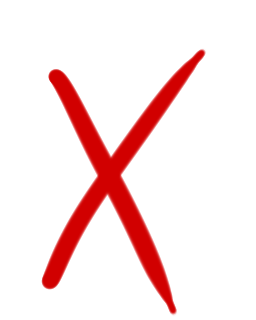
\includegraphics[scale=0.1]{no.png} &
%% 
\includegraphics[scale=0.1]{yes.png} \\

%% \end{tabular}
%% }

%% \medskip

%% \end{frame}


\begin{frame}{OSP and Our Explanation Problem in Rovers}

\centering

\begin{tikzpicture}
\node[] (task) at (-6,1) {
\begin{tikzpicture}
\node[] (p) at (0,2) {\textbf{planning task}};
\node[] (p) at (0,1.4) {soft goals};
\node[] (i1) at (-0.5,0.8) {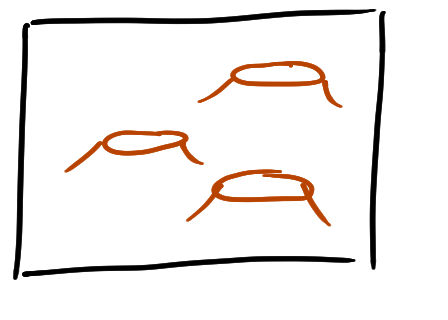
\includegraphics[scale=0.07]{rovergoal1.png}};
\node[] (i2) at (0.5,0.8) {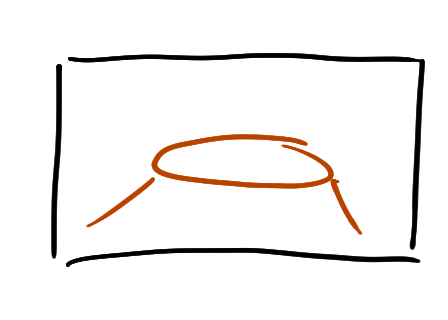
\includegraphics[scale=0.07]{rovergoal2.png}};
\node[] (i3) at (1.7,0.8) {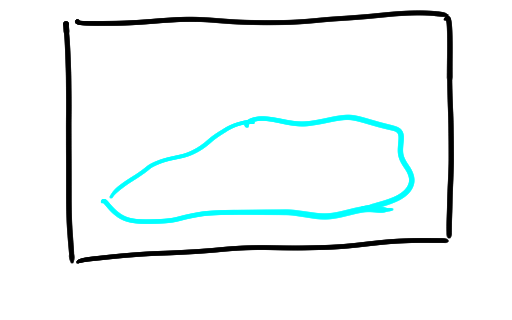
\includegraphics[scale=0.07]{rovergoal3.png}};
\node[] (r1) at (0,-0.6) {
\includegraphics[scale=0.06]{rover1.png}};
\node[] (r2) at (1.5,-0.6) {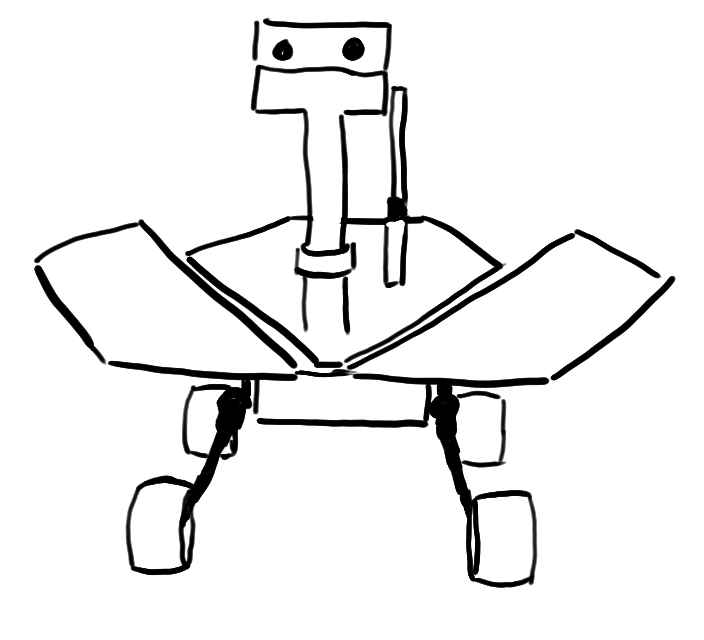
\includegraphics[scale=0.06]{rover2.png}};
\end{tikzpicture}
};

\node[] (batterylow) at (-6,-1) {
\includegraphics[scale=0.1]{battery-low.png}};

\visible<2->{
\node[] (p) at (0,2.5) {\textbf{plan}};
\node[draw, align=left, fill=white] (p1) at (0,0.9) {
$drive(R_1,L_1,L2)$\\
$takeImage(I_1, R_1)$\\
$drive(R_2,L_4,L_5)$\\
$takeImage(I_3, R_2)$
};
}

\visible<3->{
\node[fill=white] (p1) at (-0.0,-1.65) {
\begin{tabular}{c|c|c}
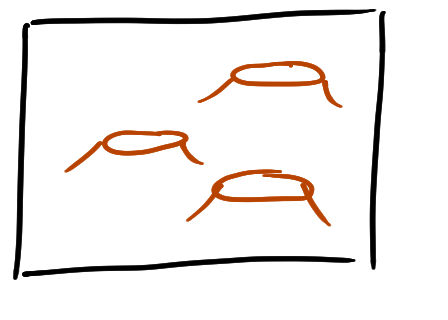
\includegraphics[scale=0.07]{rovergoal1.png} &
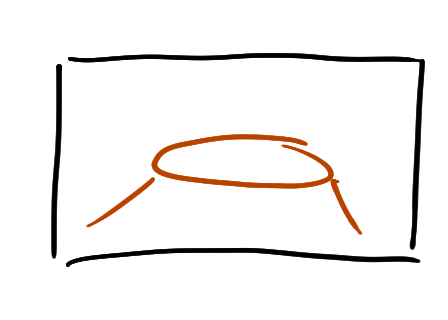
\includegraphics[scale=0.07]{rovergoal2.png} &
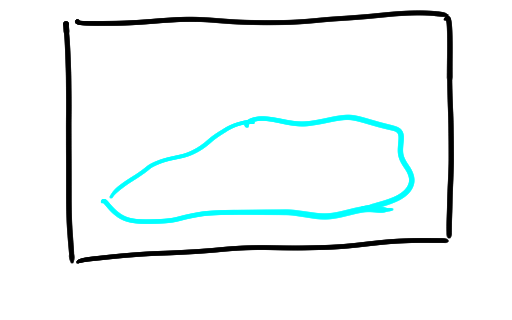
\includegraphics[scale=0.07]{rovergoal3.png} \\\hline


\includegraphics[scale=0.05]{yes.png} &
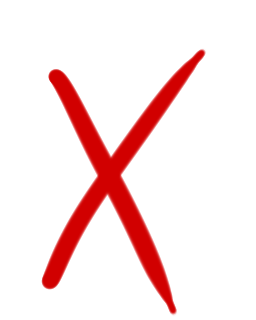
\includegraphics[scale=0.05]{no.png} &

\includegraphics[scale=0.05]{yes.png} \\

\end{tabular}
};
}

% TALK: Not putting this on slide for lack of space, but ``Why?'' of
% course here means ``Why does the plan not take image $I_2$?''
%
\visible<4>{
\node[] (hw) at (-3.7,-2.5) {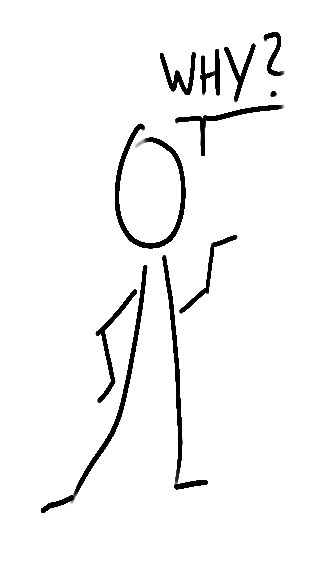
\includegraphics[scale=0.2]{human-why.png}};
}
\end{tikzpicture}
	
\end{frame}



%%%%%%%%%%%%%%%%%%%%%%%%%%%%%%%%%%%%%%%%%%%%%%%%%%%%%%%%%%%%%%%%%%%%%%%%%%%%%%%%%
%%%%%%%%%%%%%%%%%%%%%%%%%%%%%%%%%%%%%%%%%%%%%%%%%%%%%%%%%%%%%%%%%%%%%%%%%%%%%%%%%
%%%%%%%%%%%%%%%%%%%%%%%%%%%%%%%%%%%%%%%%%%%%%%%%%%%%%%%%%%%%%%%%%%%%%%%%%%%%%%%%%
%%% Explanation Framework
%
%%% Timing: XX min

\section[Framework]{Explanation Framework}
\subsection*{}

\begin{frame}{Plan Properties}

\notesym~Plan properties over soft goals in OSP:

\begin{mydef}{Plan Properties}
OSP task $\task =
(\vars,\allowbreak\acts,\allowbreak\cost,\allowbreak\init,\allowbreak\goalhard,\allowbreak\goalsoft,\allowbreak\costbound)$, \textred{\plans\
its set of plans}.
\begin{itemize}
\item  \defined{Plan property}: propositional formula $\phi$ over 
atoms $g \in \goalsoft$
\item \defined{Conjunctive} plan property: $\phi$ has form
\textred{$\bigwedge_{g \in A} g\allowbreak$} or \textred{$\neg \bigwedge_{g \in B} g$}
\end{itemize}
%
%% A \defined{plan property} is a function $\prop_\phi : \plans \mapsto
%% \{\true, \false\}$ where $\phi$ is a propositional formula over the
%% atoms \goalsoft, and $\prop_\phi(\plan) = \true$ iff $\phi$ evaluates
%% to \true\ under the truth value assignment where $g \in \goalsoft$ is
%% \true\ iff $g \in \init\apply{\plan}$.
%% %
%% $\prop_\phi$ is \defined{conjunctive} if $\phi$ has the form
%% $\bigwedge_{g \in A} g\allowbreak$ or $\neg \bigwedge_{g \in B} g$.
%
\end{mydef}

\bigskip \pause

% TALK: Explain here already that we view plan properties as functions
% from plans to Booleans: which soft goals does the plan achieve?
%
\textbf{Simple special case:} Can use arbitrary functions $\plans \to \{\true, \false\}$

\begin{itemize}
\item \eg\ temporal plan trajectory constraints
\item \eg\ deadlines, resource bounds
\end{itemize}

\medskip \pause

\textbf{Compilation:} Into (additional variables/actions and) goal facts!

\begin{itemize}
\item \eg\ LTL formulas
\item Here: action-set properties, easy special case of LTL
\end{itemize}

\medskip

\end{frame}


\begin{frame}{\plans-Entailment}

\textred{\notesym~\plans\ in the role of a knowledge base:}

\begin{mydef}{\plans-Entailment}
OSP task $\task =
(\vars,\allowbreak\acts,\allowbreak\cost,\allowbreak\init,\allowbreak\goalhard,\allowbreak\goalsoft,\allowbreak\costbound)$, \plans\
its set of \textred{plans \plan}.
\begin{itemize}
\item \defined{$\plan$ satisfies $\phi$, $\plan \models \phi$}: if $\phi$ true given truth value
assignment to $g \in \goalsoft$ defined
by \textred{$g \in \init\apply{\plan}$ ? $g \mapsto \true$ :
$g \mapsto \false$}
\item $\defined{\modelsof{\plans}{\phi}} := \{\plan \mid \plan
\in \plans, \plan \models \phi\}$
\item \defined{$\phi$ \plans-entails $\psi$, written
$\entails{\plans}{\phi}{\psi}$}: if \textred{$\modelsof{\plans}{\phi} \subseteq
\modelsof{\plans}{\psi}$}
\end{itemize}
%
%% We say that $\plan \in \plans$ \defined{satisfies} a plan property
%% $\phi$, written $\plan \models \phi$, if $\prop_\phi(\plan) =
%% \true$. We denote by $\modelsof{\plans}{\phi} := \{\plan \mid \plan
%% \in \plans, \plan \models \phi\}$ the subset of plans that satisfy
%% $\phi$.
%% %
%% %% We say that \phi\ is \defined{satisfiable} in \plans\ if
%% %% $\modelsof{\plans}{\phi} \neq \emptyset$.
%% %
%% We say that $\phi$ \defined{\plans-entails} $\psi$, written
%% $\entails{\plans}{\phi}{\psi}$, if $\modelsof{\plans}{\phi} \subseteq
%% \modelsof{\plans}{\psi}$.
%
\end{mydef}

\medskip \pause

\notesym~Special case focus here:

\begin{mydef}{Goal Exclusions}
%
\begin{itemize}
\item \defined{Goal exclusion}: entailment of form
\textred{$\entails{\plans}{\bigwedge_{g \in A} g}{\neg \bigwedge_{g \in B} g}$}
\item \defined{Non-dominated}: $\not\exists$ $(A',B') \neq
(A,B)$: \textred{$A' \subseteq A$}, \textred{$B' \subseteq B$},
  $\entails{\plans}{\bigwedge_{g \in \textred{A'}}
  g}{\neg \bigwedge_{g \in \textred{B'}} g}$
\end{itemize}
%
%% A \defined{goal exclusion} is an entailment of the form
%% $\entails{\plans}{\bigwedge_{g \in A} g}{\neg \bigwedge_{g \in B}
%%   g}$. 
%% %
%% The entailment is \defined{non-dominated} if there is no pair
%% $(A',B')$ where $A' \subseteq A$, $B' \subseteq B$, $(A',B') \neq
%% (A,B)$, and $\entails{\plans}{\bigwedge_{a \in A'} a}{\neg
%%   \bigwedge_{g \in B'} g}$.
%% %
%% The entailment is \defined{non-rhs-dominated} if there is no $B'$
%% where $B' \subsetneq B$ and $\entails{\plans}{\bigwedge_{a \in A}
%%   a}{\neg \bigwedge_{g \in B'} g}$.
%
\end{mydef}

% TALK: A non-dominated goal exclusion has subset-minimal $A$ and
% $B$. This dominates entailments with larger $A$ and/or $B$ as it has
% a weaker left-hand side $A$ (smaller conjunction) entailing a
% stronger right-hand side $\neg B$ (smaller disjunction, after moving
% the negation inside). If $A$ is fixed, then only the right-hand side
% $B$ needs be minimal. We will use non-dominated entailments to give
% more compact explanations.

\medskip

\end{frame}


\begin{frame}{\plans-Entailment: Rovers Example}

\visible<2->{

\textbf{\plans-entailment:}

\begin{tikzpicture}
\node[] (depi2) at (-6.0,2) {
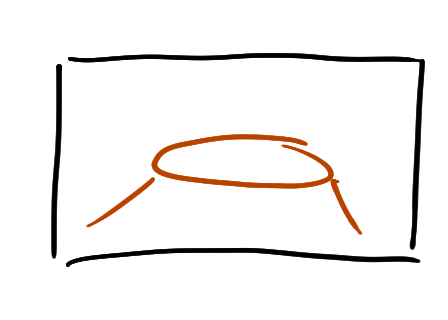
\includegraphics[scale=0.1]{rovergoal2.png} 
};
\node[] (depi23) at (-5.0,2) {$\Rightarrow$};
\node[] (depi3) at (-4.0,2) {
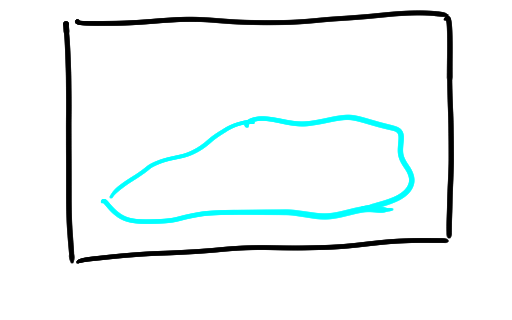
\includegraphics[scale=0.1]{rovergoal3.png}
};
\node[] (depn3) at (-4.0,2) {
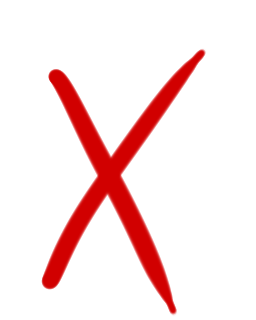
\includegraphics[scale=0.1]{no.png} 
};
%
%% \draw[thick, ->] (depi2) to (depi3);
\end{tikzpicture}

}

\visible<3->{

\textbf{Dominated \plans-entailment:}

\begin{tikzpicture}
\node[] (depi1) at (-6.0,2) {
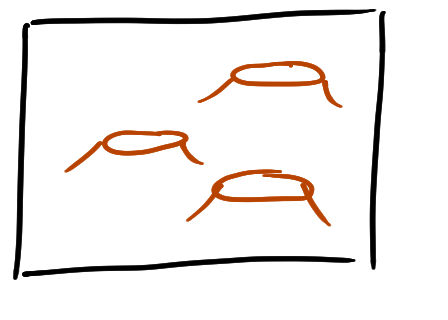
\includegraphics[scale=0.1]{rovergoal1.png} 
};
\node[] (depi2) at (-4.8,2) {
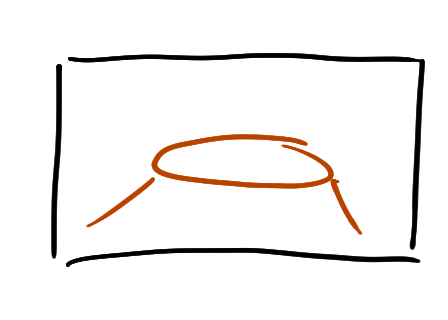
\includegraphics[scale=0.1]{rovergoal2.png} 
};
\node[] (depi23) at (-3.8,2) {$\Rightarrow$};
\node[] (depi3) at (-2.8,2) {
\includegraphics[scale=0.1]{rovergoal3.png}
};
\node[] (depn3) at (-2.8,2) {
\includegraphics[scale=0.1]{no.png} 
};

%% \draw[thick, ->] (depi2) to (depi3);
\end{tikzpicture}

}

\vspace{-2.5cm} \hfill \includegraphics[height=0.7\textheight]{rovers-example-low}

\end{frame}


\begin{frame}{Global Explanations}

% TALK: Briefly discuss straightforward def. QUESTION: Issues with
% this? Many plan properties (here: all propositional formulas over
% soft goals) and many equivalence classes (here: in the worst case,
% one class for every set of truth-value assignments to the soft
% goals).
%
\notesym~All entailment relations over plan properties in the task:

\begin{mydef}{Global Explanation (GE)}
%
OSP task $\task =
(\vars,\allowbreak\acts,\allowbreak\cost,\allowbreak\init,\allowbreak\goalhard,\allowbreak\goalsoft,\allowbreak\costbound)$, \plans\
its set of plans.
\begin{itemize}
\item \defined{$\equiv{\plans}{\phi}$}: equivalence class, \ie\ set of $\psi$ with 
$\modelsof{\plans}{\phi} = \modelsof{\plans}{\psi}$
\item \defined{Global explanation (GE) for \task}: strict partial order
over equivalence classes, $\equiv{\plans}{\phi}
< \equiv{\plans}{\psi}$ iff \textred{$\equiv{\plans}{\phi}
\neq \equiv{\plans}{\psi}$ and $\entails{\plans}{\phi}{\psi}$}
\end{itemize}
%
%% Denote by $\equiv{\plans}{\phi} := \{\psi \mid \modelsof{\plans}{\phi}
%% = \modelsof{\plans}{\psi}\}$ the \plans-equivalence class of $\phi$.
%% %
%% The \defined{global explanation (GE)} for \task\ is the strict partial
%% order $\pdo{\plans}$ over the classes $\equiv{\plans}{\phi}$ where
%% $\equiv{\plans}{\phi} \pdo{\plans} \equiv{\plans}{\psi}$ iff
%% $\equiv{\plans}{\phi} \neq \equiv{\plans}{\psi}$ and
%% $\entails{\plans}{\phi}{\psi}$.
%
\end{mydef}

\medskip \pause

% TALK: No chains of entailments here, in particular phi and psi
% cannot entail each other so no equivalence classes needed.
%
\notesym~More practical variant for goal exclusions:

\begin{mydef}{Goal-Exclusion GE}
%
OSP task $\task =
(\vars,\allowbreak\acts,\allowbreak\cost,\allowbreak\init,\allowbreak\goalhard,\allowbreak\goalsoft,\allowbreak\costbound)$, \plans\
its set of plans.
\begin{itemize}
\item \defined{goal-exclusion GE for \task}: strict partial 
order over conjunctive plan properties induced by
the \textred{non-dominated goal exclusions
$\entails{\plans}{\bigwedge_{g \in A} g}{\neg \bigwedge_{g \in B} g}$}
\end{itemize}
%
%% The \defined{goal-exclusion GE} for \task\ is the partial order
%% $\pdo{\plans}$ over conjunctive plan properties where $\phi
%% \pdo{\plans} \psi$ iff $\entails{\plans}{\phi}{\psi}$ is a
%% non-dominated goal exclusion.
%
\end{mydef}

\medskip

\end{frame}


\begin{frame}{Goal-Exclusion GE: Rovers Example}

% TALK: Brief forward reference to MUGS.
%
\visible<2->{

\textbf{All non-dominated goal exclusions:}

\begin{tikzpicture}
\node[] (depi2) at (-6.0,2) {
\includegraphics[scale=0.1]{rovergoal2.png} 
};
\node[] (depi23) at (-5.0,2) {$\Rightarrow$};
\node[] (depi3) at (-4.0,2) {
\includegraphics[scale=0.1]{rovergoal3.png}
};
\node[] (depn3) at (-4.0,2) {
\includegraphics[scale=0.1]{no.png} 
};
%
%% \draw[thick, ->] (depi2) to (depi3);
\end{tikzpicture}

\vspace{-0.3cm} \begin{tikzpicture}
\node[] (depi2) at (-6.0,2) {
\includegraphics[scale=0.1]{rovergoal3.png} 
};
\node[] (depi23) at (-5.0,2) {$\Rightarrow$};
\node[] (depi3) at (-4.0,2) {
\includegraphics[scale=0.1]{rovergoal2.png}
};
\node[] (depn3) at (-4.0,2) {
\includegraphics[scale=0.1]{no.png} 
};
%
%% \draw[thick, ->] (depi2) to (depi3);
\end{tikzpicture}

}

\vspace{-1.7cm} \hfill \includegraphics[height=0.7\textheight]{rovers-example-low}

\end{frame}


\begin{frame}{Local Explanations}

\notesym~In response to user question ``Why not property $\phi$?'':

\begin{mydef}{Local Explanation (LE)}
%
OSP task $\task =
(\vars,\allowbreak\acts,\allowbreak\cost,\allowbreak\init,\allowbreak\goalhard,\allowbreak\goalsoft,\allowbreak\costbound)$, \plans\
its set of plans.
\begin{itemize}
\item \defined{Local explanation (LE) for $\phi$}: 
$\{\psi \mid \entails{\plans}{\phi}{\psi}\}$
\item \defined{Goal-exclusion LE for $\phi = \bigwedge_{g \in A} g$}: $\{\psi \mid \psi = \neg \bigwedge_{g \in B} g,
\entails{\plans}{\phi}{\psi} \text{ is non-rhs-dominated}\}$\pause
\item \defined{Non-rhs-dominated}: $\not\exists$ $B'$: \textred{$B' \subsetneq B$},
  $\entails{\plans}{\bigwedge_{g \in A}
  g}{\neg \bigwedge_{g \in \textred{B'}} g}$
\end{itemize}
%
%% For a plan property $\phi$, the \defined{local explanation (LE)} for
%% $\phi$ is the set $\{\psi \mid \entails{\plans}{\phi}{\psi}\}$ of plan
%% properties \plans-entailed by $\phi$.
%% %
%% For $\phi = \bigwedge_{g \in A} g$, the \defined{goal-exclusion LE}
%% for $\phi$ is $\{\psi \mid \psi = \neg \bigwedge_{g \in B} g,
%% \entails{\plans}{\phi}{\psi} \text{ is non-rhs-dominated}\}$.
%
%% The entailment is \defined{non-rhs-dominated} if there is no $B'$
%% where $B' \subsetneq B$ and $\entails{\plans}{\bigwedge_{g \in A}
%%   g}{\neg \bigwedge_{g \in B'} g}$.
%
\end{mydef}

\bigskip \pause

\textbf{Remarks:} 

\begin{itemize}
\item Smaller and easier to compute than GE (see next section).
\item Relative to current plan \plan\ in iterative planning: only those 
$\psi$ where $\plan \not\models \psi$ (\ie\ new properties entailed by
$\phi$).
\end{itemize}

\medskip

\end{frame}


\begin{frame}{Goal-Exclusion LE: Rovers Example}

\only<1|handout:0>{

\centering

\begin{tikzpicture}
\node[] (task) at (-6,1) {
\begin{tikzpicture}
\node[] (p) at (0,2) {\textbf{planning task}};
\node[] (p) at (0,1.4) {soft goals};
\node[] (i1) at (-0.5,0.8) {\includegraphics[scale=0.07]{rovergoal1.png}};
\node[] (i2) at (0.5,0.8) {\includegraphics[scale=0.07]{rovergoal2.png}};
\node[] (i3) at (1.7,0.8) {\includegraphics[scale=0.07]{rovergoal3.png}};
\node[] (r1) at (0,-0.6) {\includegraphics[scale=0.06]{rover1.png}};
\node[] (r2) at (1.5,-0.6) {\includegraphics[scale=0.06]{rover2.png}};
\end{tikzpicture}
};

\node[] (batterylow) at (-6,-1) {\includegraphics[scale=0.1]{battery-low.png}};

\node[] (p) at (0,2.5) {\textbf{plan}};
\node[draw, align=left, fill=white] (p1) at (0,0.9) {
$drive(R_1,L_1,L2)$\\
$takeImage(I_1, R_1)$\\
$drive(R_2,L_4,L_5)$\\
$takeImage(I_3, R_2)$
};

\node[fill=white] (p1) at (-0.0,-1.65) {
\begin{tabular}{c|c|c}
\includegraphics[scale=0.07]{rovergoal1.png} &
\includegraphics[scale=0.07]{rovergoal2.png} &
\includegraphics[scale=0.07]{rovergoal3.png} \\\hline

\includegraphics[scale=0.05]{yes.png} &
\includegraphics[scale=0.05]{no.png} &
\includegraphics[scale=0.05]{yes.png} \\

\end{tabular}
};

\node[] (hw) at (-3.7,-2.5) {\includegraphics[scale=0.2]{human-why.png}};
\end{tikzpicture}

}%
%
\only<2-|handout:1>{

\textbf{Why does this plan not achieve \hspace{1.4cm}?}

\vspace{-0.9cm} \hspace{5.3cm} \begin{tikzpicture}
\node[] (depi2) at (-6.0,2) {
\includegraphics[scale=0.1]{rovergoal2.png} 
};
\end{tikzpicture}

\vspace{-0.2cm}

Because  

\vspace{-0.8cm} \hspace{1.05cm} \begin{tikzpicture}
\node[] (depi2) at (-6.0,2) {
\includegraphics[scale=0.1]{rovergoal2.png} 
};
\node[] (depi23) at (-5.0,2) {$\Rightarrow$};
\node[] (depi3) at (-4.0,2) {
\includegraphics[scale=0.1]{rovergoal3.png}
};
\node[] (depn3) at (-4.0,2) {
\includegraphics[scale=0.1]{no.png} 
};
\end{tikzpicture}

\vspace{-0.55cm} \hfill \includegraphics[height=0.7\textheight]{rovers-example-low}

}

\end{frame}


\begin{frame}{Another Example: Transportation (IPC ``NoMystery'')}

{\centering

\begin{tabular}{cc}
\begin{minipage}{0.35\textwidth}
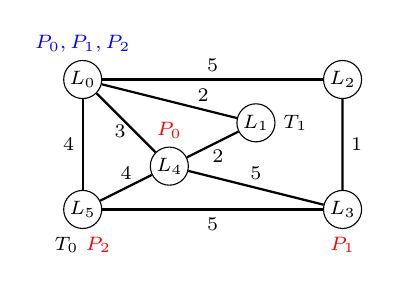
\begin{tikzpicture}[scale=0.55]
	\scriptsize
  \node[draw, circle, inner sep=1pt, label=above:{\textcolor{blue}{$P_0, P_1,P_2$}}] (l0) at (0,0) {$L_0$};
  \node[draw, circle, inner sep=1pt, label=right:{$T_1$}] (l1) at (4,-1) {$L_1$};
  \node[draw, circle, inner sep=1pt] (l2) at (6,0) {$L_2$};
  \node[draw, circle, inner sep=1pt, label=below:{\textcolor{red}{$P_1$}}] (l3) at (6,-3) {$L_3$};
  \node[draw, circle, inner sep=1pt, label=above:{\textcolor{red}{$P_0$}}] (l4) at (2,-2) {$L_4$};
  \node[draw, circle, inner sep=1pt, label=below:{$T_0$ \textcolor{red}{$P_2$}}] (l5) at (0,-3) {$L_5$};

  \draw[thick] (l0) to node[above] {5} (l2);
  \draw[thick] (l0) to node[above, pos=0.75] {2} (l1);
  \draw[thick] (l0) to node[below, pos=0.4] {3} (l4);
  \draw[thick] (l0) to node[left] {4} (l5);
  \draw[thick] (l2) to node[right] {1} (l3);
  \draw[thick] (l4) to node[below, pos=0.6] {2} (l1);
  \draw[thick] (l4) to node[above] {5} (l3);
  \draw[thick] (l5) to node[below] {5} (l3);
  \draw[thick] (l4) to node[above] {4} (l5);
\end{tikzpicture}
\end{minipage} &
\hspace{-0.4cm} \begin{minipage}{0.56\textwidth}
\scriptsize

\begin{itemize}
\item Variables \vars: $T_1, f_1, T_2, f_2, P_0, P_1, P_2$
\item Actions \acts: $drive(T_i,L_x,L_y)$, $load(T_i,P_j,L_x)$, $unload(T_i,P_j,L_x)$

      Driving consumes fuel as indicated
\item Initial state \init: as shown; \textred{$\init(f_1)=13, \init(f_2)=0$}
\item Goal \goalsoft: $at(P_0,L_4), at(P_1,L_3), at(P_2,L_5)$
\end{itemize}

\end{minipage}
\end{tabular}

}

\bigskip \pause

\textbf{Non-dominated goal exclusions:} 

\pause \prehandout{\bigskip\bigskip\bigskip\bigskip\bigskip\bigskip} \noprehandout{

\begin{itemize}
\item $\entails{\plans}{P_0}{\neg (P_1 \wedge P_2)}$
\item $\entails{\plans}{P_1}{\neg (P_0 \wedge P_2)}$
\item $\entails{\plans}{P_2}{\neg (P_0 \wedge P_1)}$
\end{itemize}

\pause

\notesym~In other words: ``\goalsoft\ is not solvable 
as a whole, but each of its subsets is''.

}

\medskip

\end{frame}



%%%%%%%%%%%%%%%%%%%%%%%%%%%%%%%%%%%%%%%%%%%%%%%%%%%%%%%%%%%%%%%%%%%%%%%%%%%%%%%%%
%%%%%%%%%%%%%%%%%%%%%%%%%%%%%%%%%%%%%%%%%%%%%%%%%%%%%%%%%%%%%%%%%%%%%%%%%%%%%%%%%
%%%%%%%%%%%%%%%%%%%%%%%%%%%%%%%%%%%%%%%%%%%%%%%%%%%%%%%%%%%%%%%%%%%%%%%%%%%%%%%%%
%%% Computing Explanations
%
%%% Timing: XX min

\section[Computing]{Computing Explanations}
\subsection*{}

\begin{frame}{Non-Dominated Goal Exclusions from MUGS}

\begin{mydef}{Minimal Unsolvable Goal Subset (MUGS)}
%
OSP task $\task =
(\vars,\allowbreak\acts,\allowbreak\cost,\allowbreak\init,\allowbreak\goalhard,\allowbreak\goalsoft,\allowbreak\costbound)$, \plans\
its set of plans.
\begin{itemize}
\item \defined{Minimal unsolvable goal subset (MUGS)}: unsolvable 
$\goal \subseteq \goalsoft$, every $\goal' \subsetneq \goal$ solvable
\end{itemize}
%
\end{mydef}

\medskip \pause

% TALK: Previous defs somewhat of an overkill given it all boils down
% to MUGS. But: this is so only in the special case of goal
% exclusions. In general, plan-property dependencies always equivalent
% to unsat of conjunction as always for entailment; but not
% necessarily a more compact formulation in the form of conflict sets
% as here.
%
\begin{myprop}{Non-dominated Goal Exclusions from MUGS}
%
\textred{Non-dominated $\entails{\plans}{\bigwedge_{g \in A} g}{\neg \bigwedge_{g \in B} g}$
  $\Leftrightarrow$ $A \cup B$ MUGS}
%
\end{myprop}

\vspace{-0.1cm}

\begin{proof}
%
A \plans-entailment $\entails{\plans}{\bigwedge_{g \in A} g}{\neg
  \bigwedge_{g \in B} g}$ clearly holds iff $A \cup B$ is
unsolvable. Non-dominated entailments result from set-inclusion
minimal $A$ and $B$, corresponding to the set-inclusion minimality of
MUGS.
%
\end{proof}

\notesym~Compute and represent goal-exclusion GE via MUGs.

\medskip

\end{frame}


\begin{frame}{Systematic Weakening}

\vspace{-0.2cm}

\begin{enumerate}
\item Start with \goalsoft 
\item Select open node $\goal$, call planner
  to test solvability, cache result, expand $\goal$ if unsolvable
\item children of $\goal$: $\goal' \subset \goal$ where $|\goal'| = |\goal|-1$
\end{enumerate}

\smallskip

{\centering

\begin{tikzpicture}
\visible<1>{
\node[draw] (all) at (0,5) {\rovergoal{1} \rovergoal{2} \rovergoal{3}};
}
\visible<2->{
\node[draw, fill=mLightBrown!40] (all) at (0,5) {\rovergoal{1} \rovergoal{2} \rovergoal{3}};
}

\visible<3>{
\node[draw] (01) at (-3,3) {\rovergoal{1} \rovergoal{2}};
\node[draw] (02) at (0,3) {\rovergoal{1} \rovergoal{3}};
\node[draw] (12) at (3,3) {\rovergoal{2} \rovergoal{3}};
}
\visible<4-6>{
\node[draw, fill=mLightBrown!40] (01) at (-3,3) {\rovergoal{1} \rovergoal{2}};
\node[draw, fill=mLightGreen!40] (02) at (0,3) {\rovergoal{1} \rovergoal{3}};
\node[draw, fill=mLightBrown!40] (12) at (3,3) {\rovergoal{2} \rovergoal{3}};
}
\visible<7->{
\node[draw, fill=mLightBrown!40, line width=2pt] (01) at (-3,3) {\rovergoal{1} \rovergoal{2}};
\node[draw, fill=mLightGreen!40] (02) at (0,3) {\rovergoal{1} \rovergoal{3}};
\node[draw, fill=mLightBrown!40, line width=2pt] (12) at (3,3) {\rovergoal{2} \rovergoal{3}};
}

\visible<5>{
\node[draw] (0) at (-2,1) {\rovergoal{1}};
\node[draw] (1) at (0,1) {\rovergoal{2}};
\node[draw] (2) at (2,1) {\rovergoal{3}};
}	
\visible<6->{
\node[draw, fill=mLightGreen!40] (0) at (-2,1) {\rovergoal{1}};
\node[draw, fill=mLightGreen!40] (1) at (0,1) {\rovergoal{2}};
\node[draw, fill=mLightGreen!40] (2) at (2,1) {\rovergoal{3}};
}

\visible<3->{
\draw[thick, ->] (all) to (01);
\draw[thick, ->] (all) to (02);
\draw[thick, ->] (all) to (12);
}
\visible<5->{
\draw[thick, ->] (01) to (0);
\draw[thick, ->] (01) to (1);
\draw[thick, ->] (12) to (2);
}
\end{tikzpicture}

}

\medskip\smallskip

\end{frame}


\begin{frame}{Experiments: Global Explanations}

\centering

\setlength{\tabcolsep}{2pt}
\renewcommand{\arraystretch}{0.8}

\tiny

\begin{tabular}{l||r|rrr||rr|rr|rr||rr|rr||rrr}
& \multicolumn{4}{c||}{Reference Coverage}  & \multicolumn{6}{c||}{SysS/W Coverage} & \multicolumn{4}{c||}{Search Fraction} & \multicolumn{3}{c}{\#MUGS, $x=$} \\
& \hlmcut & \multicolumn{3}{c||}{OSP} & \multicolumn{2}{c|}{0.25} & \multicolumn{2}{c|}{0.5} & \multicolumn{2}{c||}{0.75} & \multicolumn{2}{c|}{0.25} & \multicolumn{2}{c||}{0.75} & \multicolumn{3}{c}{average} \\
domain & & 0.25& 0.5&0.75& S & W & S & W & S & W & S & W & S & W & 0.25 & 0.5 & 0.75\\\hline\hline
agricola (20)          & 0 & 0 & 0 & 0 & 20 & 20 & 13 & 13 & 1 & 1 & 1 & 0.5 & 1 & 0.5 & 1 & 1 & 1 \\
airport (50)           & 28 & 28 & 24 & 22 & 35 & 34 & 21 & 21 & 16 & 16 & 0.6 & 0.81 & 1 & 0.61 & 3.8 & 2 & 1.4 \\
barman (34)            & 4 & 18 & 11 & 4 & 18 & 18 & 4 & 4 & 3 & 4 & 0.57 & 0.94 & 1 & 0.5 & 6.9 & 4.2 & 2.5 \\
blocks (35)            & 28 & 35 & 28 & 21 & 35 & 35 & 29 & 29 & 26 & 26 & 0.15 & 0.97 & 0.8 & 0.64 & 11 & 12.4 & 13.7 \\
childsnack (20)        & 0 & 2 & 0 & 0 & 4 & 4 & 0 & 0 & 0 & 0 & 0.34 & 0.98 &    -      &     -     & 16.8 &    -      &   -   \\
data-network (20)      & 12 & 13 & 13 & 13 & 20 & 20 & 18 & 18 & 17 & 15 & 0.72 & 0.73 & 0.91 & 0.66 & 2.1 & 1.8 & 1.5 \\
depot (22)             & 7 & 16 & 11 & 7 & 16 & 16 & 9 & 10 & 3 & 3 & 0.24 & 0.96 & 0.89 & 0.68 & 8.3 & 7 & 6.5 \\
driverlog (20)         & 13 & 15 & 13 & 10 & 15 & 15 & 12 & 12 & 10 & 10 & 0.17 & 0.98 & 0.87 & 0.5 & 8.1 & 16.1 & 11.1 \\
elevators (50)         & 40 & 22 & 22 & 22 & 47 & 48 & 38 & 37 & 27 & 27 & 0.35 & 0.94 & 0.9 & 0.67 & 4.6 & 5.1 & 5.9 \\
floortile (36)         & 13 & 18 & 6 & 2 & 8 & 8 & 2 & 2 & 2 & 2 & 0.1 & 0.99 & 0.96 & 0.3 & 316.2 & 137 & 45.5 \\
freecell (80)          & 15 & 77 & 30 & 21 & 76 & 76 & 30 & 30 & 18 & 18 & 0.31 & 0.94 & 0.88 & 0.76 & 4 & 4.3 & 3.3 \\
ged (20)               & 15 & 20 & 20 & 20 & 16 & 20 & 10 & 12 & 7 & 7 & 0.25 & 0.9 & 0.58 & 0.7 & 13.3 & 38.7 & 12.5 \\
grid (5)               & 2 & 5 & 3 & 2 & 5 & 5 & 3 & 4 & 3 & 3 & 0.54 & 0.84 & 1 & 0.54 & 4 & 2.5 & 1 \\
gripper (20)           & 7 & 11 & 8 & 8 & 5 & 5 & 4 & 4 & 3 & 3 & 0.21 & 0.98 & 0.96 & 0.46 & 783.5 & 228 & 156 \\
hiking (20)            & 9 & 19 & 14 & 13 & 20 & 20 & 16 & 17 & 11 & 10 & 0.81 & 0.69 & 1 & 0.63 & 1.8 & 1.7 & 1 \\
logistics (60)         & 26 & 27 & 20 & 16 & 15 & 15 & 6 & 6 & 3 & 4 & 0.35 & 0.95 & 0.98 & 0.73 & 7.2 & 7.3 & 2.8 \\
miconic (150)          & 141 & 97 & 66 & 55 & 66 & 64 & 42 & 43 & 35 & 36 & 0.3 & 0.92 & 0.95 & 0.61 & 81.3 & 38.2 & 18.8 \\
mprime (35)            & 22 & 35 & 27 & 24 & 35 & 35 & 35 & 35 & 35 & 35 & 0.9 & 0.59 & 0.94 & 0.59 & 1.3 & 1.2 & 1.1 \\
mystery (30)           & 12 & 29 & 27 & 21 & 30 & 30 & 30 & 30 & 30 & 30 & 0.89 & 0.61 & 0.93 & 0.61 & 1.3 & 1.2 & 1.1 \\
nomystery (20)         & 14 & 20 & 14 & 10 & 20 & 20 & 12 & 12 & 8 & 8 & 0.15 & 0.98 & 0.87 & 0.61 & 20.2 & 18.5 & 5.8 \\
openstacks (77)        & 47 & 63 & 56 & 52 & 49 & 43 & 45 & 39 & 42 & 35 & 0.03 & 0.99 & 0.12 & 0.98 & 15.3 & 14.9 & 10.3 \\
organic-syn-s (13)     & 10 & 8 & 8 & 8 & 8 & 8 & 8 & 8 & 6 & 6 & 0.19 & 0.96 & 0.28 & 0.91 & 5.3 & 7.3 & 8.3 \\
parcprinter (26)       & 24 & 26 & 22 & 18 & 10 & 14 & 10 & 14 & 10 & 12 & 0.44 & 0.98 & 0.73 & 0.85 & 5.6 & 7.5 & 4.1 \\
parking (40)           & 5 & 25 & 5 & 0 & 17 & 12 & 1 & 1 & 0 & 0 & 0.02 & 1 &   -       &   -       & 63.9 & 31 &      \\
pathways (30)          & 5 & 5 & 4 & 4 & 7 & 7 & 5 & 5 & 4 & 4 & 0.41 & 0.86 & 0.91 & 0.7 & 11.3 & 3.8 & 1.8 \\
pegsol (2)             & 2 & 2 & 2 & 2 & 0 & 2 & 0 & 2 & 0 & 2 &    -      &    -      &    -      &    -      & 7 & 23.5 & 64 \\
pipesworld-nt (50)     & 17 & 45 & 30 & 23 & 46 & 46 & 25 & 26 & 15 & 15 & 0.31 & 0.94 & 0.88 & 0.66 & 5 & 5.6 & 4.3 \\
pipesworld-t (50)      & 12 & 33 & 20 & 16 & 39 & 40 & 18 & 17 & 13 & 11 & 0.35 & 0.95 & 0.88 & 0.65 & 4 & 4.2 & 3.2 \\\hline
Sum (1517)             & 828 & 1088 & 828 & 705 & 1026 & 1005 & 690 & 694 & 522 & 528 &      &      &      &      &      &      &      \\
\end{tabular}
 

\end{frame}


\begin{frame}{Local Explanations from MUGS}

\notesym~In response to user question ``Why not property $\bigwedge_{g \in A} g$?'':

\begin{myprop}{Non-rhs-dominated Goal Exclusions from MUGS}
%
OSP task $\task =
(\vars,\allowbreak\acts,\allowbreak\cost,\allowbreak\init,\allowbreak\goalhard,\allowbreak\goalsoft,\allowbreak\costbound)$, \plans\
its set of plans.

Modified task $\task' :=
(\vars,\allowbreak\acts,\allowbreak\cost,\allowbreak\init,\allowbreak\textred{\goalhard
\cup A},\allowbreak\textred{\goalsoft \setminus
A},\allowbreak\costbound)$.

Then: \textred{Non-rhs-dominated $\entails{\plans}{\bigwedge_{g \in A}
  g}{\neg \bigwedge_{g \in B} g}$ $\Leftrightarrow$ $B$ MUGS in
  $\task'$}.
%
\end{myprop}

\bigskip \smallskip \pause

% TALK: Why is this easier than before?
%
\textbf{This is easier \& smaller because:} \pause \prehandout{\bigskip\bigskip\bigskip\bigskip} \noprehandout{Less soft goals!

\begin{itemize}
\item Search tree size worst-case exponential in $|\goalsoft|$
\item \#MUGS worst-case exponential in $|\goalsoft|$
\end{itemize}

}

\medskip

\end{frame}


\begin{frame}{Experiments: Local Explanations}

\notesym~Performance and \#MUGS \textred{as function of question size $|A|$}
in ``Why not property $\bigwedge_{g \in A} g$?'':

\medskip

\small

\centering

\begin{tabular}{cc}
\begin{minipage}{0.45\textwidth}
\includegraphics[height=4.2cm]{plot-ipc-performance.png}
\end{minipage} &
\hspace{0.5cm} \begin{minipage}{0.45\textwidth}
\includegraphics[height=4.2cm]{plot-ipc-mugs.png}
\end{minipage}
\end{tabular}

\end{frame}



%%%%%%%%%%%%%%%%%%%%%%%%%%%%%%%%%%%%%%%%%%%%%%%%%%%%%%%%%%%%%%%%%%%%%%%%%%%%%%%%%
%%%%%%%%%%%%%%%%%%%%%%%%%%%%%%%%%%%%%%%%%%%%%%%%%%%%%%%%%%%%%%%%%%%%%%%%%%%%%%%%%
%%%%%%%%%%%%%%%%%%%%%%%%%%%%%%%%%%%%%%%%%%%%%%%%%%%%%%%%%%%%%%%%%%%%%%%%%%%%%%%%%
%%% Compilations
%
%%% Timing: XX min

\section[Compilations]{Compilations}
\subsection*{}

\begin{frame}{We Want More General Plan Properties!}

\centering

\begin{tikzpicture}
\node[] (task) at (0,-0.7) {
\resizebox{!}{5cm}{%
\begin{tikzpicture}
\node[] (t) at (1.5,2) {\includegraphics[scale=0.07]{rover2.png}};
\node[] (t) at (-5,-2.5) {\includegraphics[scale=0.07]{rover1.png}};

\node[] (m) at (0,0) {\includegraphics[scale=0.2]{mars.png}};

\node[draw, circle, inner sep=3pt] (l1) at (-3,-3) {$L_1$};
\node[draw, circle, inner sep=3pt] (l2) at (-2.1,1.3) {$L_2$};
\node[draw, circle, inner sep=3pt] (l3) at (-0.5,-1) {$L_3$};
\node[draw, circle, inner sep=3pt] (l4) at (3,2) {$L_4$};
\node[draw, circle, inner sep=3pt] (l5) at (1.8,0) {$L_5$};
\node[draw, circle, inner sep=3pt] (l6) at (3.2,-2.5) {$L_6$};

\draw[thick] (l1) to (l2);
\draw[thick] (l1) to (l3);
\draw[thick] (l2) to (l3);
\draw[thick] (l3) to (l5);
\draw[thick] (l4) to (l5);
\draw[thick] (l4) to (l6);
\draw[thick] (l5) to (l6);
\visible<2->{
\draw[thick, red, ->, line width=0.1cm] (l1) to (l2);
\draw[thick, mLightGreen, ->, line width=0.1cm] (l1) to (l3);
\draw[thick, mLightGreen, ->, line width=0.1cm] (l3) to (l2);
}

\node[] (g) at (-1.9,-4) {\Large \textbf{goal}:};
\node[] (i1) at (-0.5,-4) {\includegraphics[scale=0.1]{rovergoal1.png}};
\node[] (i2) at (0.8,-4) {\includegraphics[scale=0.1]{rovergoal2.png}};
\node[] (i3) at (2.5,-4) {\includegraphics[scale=0.1]{rovergoal3.png}};
\end{tikzpicture}
}
};

\node[draw, align=left, fill=white] (plan) at (-1,3) {
\scriptsize
$drive(R_1,L_1,L2)$\\[-0.2cm]
\scriptsize
$takeImage(I_1,R_1)$\\[-0.2cm]
\scriptsize
$drive(R_2,L_4,L_5)$\\[-0.2cm]
\scriptsize
$takeImage(I_3,R_2)$\\[-0.2cm]
\scriptsize
$drive(R_2,L_5,L_6)$\\[-0.2cm]
\scriptsize
$takeImage(I_2,R_2)$
};

\node[] (human_why) at (-4,1.5) {\includegraphics[scale=0.2]{human-why.png}};
\node[] (ai_exp) at (4,1.5) {\includegraphics[scale=0.2]{robot-exp.png}};

\visible<3->{
\node[] (p) at (4,3.5) {
\resizebox{!}{1.5cm}{%
\begin{tikzpicture}
\node[draw, inner sep=1pt] (p1) at (0.2,0) {
\dontuseconnection{1}{1}{2}
};
\node[] (depp1p2) at (2.7,0) {\Huge $\Rightarrow$};
\node[draw, inner sep=1pt] (p2) at (5,0) {
\specificrover{1}{1}
};
\node[] (no) at (5,0.9) {\includegraphics[scale=0.1]{no.png}}; 
%\draw[thick, ->] (p1) to (p2);
\end{tikzpicture}
}
};
}

\end{tikzpicture}

\end{frame}


\begin{frame}{Compilation!}

\notesym~Compile more general plan properties into (additional 
variables/actions and) goal facts! For example:

\begin{itemize}
\item Precondition and goal formulas, conditional effects 
{\footnotesize [\cite{gazen:knoblock:ecp-97,nebel:jair-00}]}
\item LTL formulas over plan trajectory {\footnotesize [\cite{edelkamp:icaps-06,baier:etal:ai-09}]}
\item Initial state uncertainty {\footnotesize [\cite{palacios:geffner:jair-09}]}
\end{itemize}

\medskip \pause

% TALK: Also implemented LTL already, performance Ok optimizations in
% the making.
%
\notesym~Here: effective-to-compile special case of LTL

\begin{mydef}{Action-Set Properties}
%
OSP task $\task =
(\vars,\allowbreak\acts,\allowbreak\cost,\allowbreak\init,\allowbreak\goalhard,\allowbreak\goalsoft,\allowbreak\costbound)$, \plans\
its set of plans, \textred{$\acts_1, \dots, \acts_n
\subseteq \acts$}.
\begin{itemize}
\item \defined{Action-set property}: propositional formula $\phi$ over 
atoms $\acts_1, \dots, \acts_n$
\item \defined{$\plan \models \phi$}: if $\phi$ true given truth value
assignment \textred{$\acts_i \cap \{a_1, \dots, a_k\} \neq \emptyset$
?  $\acts_i \mapsto \true$ : $\acts_i \mapsto \false$} where $\plan
= \langle a_1, \dots, a_k\rangle$
\end{itemize}
%
%% An \defined{action-set property} for \task\ and $\acts_1, \dots,
%% \acts_n$ is a function $\prop_\phi : \plans \to \{\true, \false\}$
%% where $\phi$ is a propositional formula over the atoms $\acts_1,
%% \dots, \acts_n$, and $\prop_\phi(\plan) = \true$ iff $\phi$ evaluates
%% to \true\ under the truth value assignment where $\acts_i$ is
%% \true\ iff $\plan$ contains at least one action from $\acts_i$.
%
\end{mydef}

\medskip

\end{frame}


\begin{frame}{Rovers Action-Set Properties}

\centering

% TALK: Energy limit compilation: actins take fuel-level
% parameters. Order can also esily be compiled (e.g. goal fact set
% when left image is taken while right image has not yet been taken).
%
\begin{tikzpicture}
\node[draw,inner sep=2pt] (p1) at (-0.5,-3.5) {\samerover{1}{2}};
\node[draw,inner sep=2pt] (p3) at (3,-3.5) {\energylimit{1}};
\node[] (p2) at (6.5,-3.5) {\orderprop{1}{2}};
\node[] (p5no) at (6.5,-3.5) {
\includegraphics[scale=0.2]{no.png} 
};
\node[draw,inner sep=2pt] (p4) at (-0.5,0) {\specificrover{1}{2}};
\node[draw,inner sep=2pt] (p5) at (3,0) {\useconnection{1}{x}{y}};
\node[draw,inner sep=2pt] (p6) at (6.5,0) {\dontuseconnection{1}{x}{y}};
\end{tikzpicture}

\end{frame}


\begin{frame}{Rovers Action-Set Properties: ``Same Rover''}

\centering

\begin{tikzpicture}
\node[draw] (p1) at (-1,-0.7) {
\resizebox{!}{2cm}{%
\samerover{1}{2}
}
};

\visible<2->{
\node[] (s1) at (1.0,1.5) {\Large Action sets:};
\node[] (s2) at (1.0,-3.0) {\Large Test formula:};
}

\visible<3->{
\node[] (r1) at (3.5,1.5) {\includegraphics[scale=0.05]{rover1.png}};
\node[align=left] (actionsr0) at (6.5,1.5) {
$A_1 = \{takeImage(I_1,R_1),$\\
$takeImage(I_2,R_1)\}$
};

\node[] (r2) at (3.5,-0.5) {\includegraphics[scale=0.05]{rover2.png}};
\node[align=left] (actionsr1) at (6.5,-0.5) {
$A_2 = \{takeImage(I_1,R_2),$\\
$takeImage(I_2,R_2)\}$
};
}

\visible<4->{
\node[] (s2) at (5,-3.0) {\huge $A_1 \otimes A_2$};
}
\end{tikzpicture}

\end{frame}


\begin{frame}{Action-Set Property Compilation}

\textbf{Given:} \task, \plans, and $\acts_1, \dots, \acts_n$

\bigskip

\textbf{Construct:} $\task'$

\begin{itemize}
\item Booleans \textred{$\mathit{isUsed}_i$}, initially
  \false, set to \true\ by any action from $\acts_i$;
\item formula-evaluation state variables and actions
  evaluating each $\prop_\phi$ based on these, setting Boolean flags
  \textred{$\mathit{isTrue}_\phi$};
\item separate 1.\ \textred{planning phase}
  vs.\ 2.\ \textred{formula-evaluation phase}, switch action from 1.\ to
  2.\ enabled when \goalhard\ is satisfied.
\end{itemize}

\pause

$\Rightarrow$ planning-phase prefixes in $\task'$ one-to-one $\plans$;
given such prefix $\plan$, evaluation phase in $\task'$ can achieve
$\mathit{isTrue}_\phi$ iff $\plan \models \phi$.

\end{frame}


\begin{frame}{Rovers ``Same Rover'' Compilation: Illustration}

\begin{center}
\begin{tikzpicture}
\only<1-3>{
\node[align=left] (actionsr0) at (-1,1.5) {
$A_1 = \{takeImage(I_1,R_1),$\\
$takeImage(I_2,R_1)\}$
};
}
\only<4-5>{
\node[align=left, mLightGreen] (actionsr0) at (-1,1.5) {
$A_1 = \{takeImage(I_1,R_1),$\\
$takeImage(I_2,R_1)\}$
};
}
\only<6->{
\node[align=left] (actionsr0) at (-1,1.5) {
$A_1 = \{takeImage(I_1,R_1),$\\
$takeImage(I_2,R_1)\}$
};
}

\only<1-6>{
\node[align=left] (actionsr1) at (-1,-0.5) {
$A_2 = \{takeImage(I_1,R_2),$\\
$takeImage(I_2,R_2)\}$
};
}
\only<7-8>{
\node[align=left, mLightGreen] (actionsr1) at (-1,-0.5) {
$A_2 = \{takeImage(I_1,R_2),$\\
$takeImage(I_2,R_2)\}$
};
}
\only<9->{
\node[align=left] (actionsr1) at (-1,-0.5) {
$A_2 = \{takeImage(I_1,R_2),$\\
$takeImage(I_2,R_2)\}$
};
}

\node[] (formula) at (-1,-3.1) {\huge $A_1 \otimes A_2$};


\visible<2->{
\node[draw, minimum height=3.5cm, minimum width=3cm, fill=white] (p3) at (5.4,0.4) {};
\node[draw, minimum height=3.5cm, minimum width=3cm, fill=white] (p2) at (5.2,0.2) {};
\node[draw, align=left, fill=white] (p1) at (5,0) {
$drive(R_1,L_1,L2)$\\
\only<-3|handout:1>{$takeImage(I_1,R_1)$}\only<4-5|handout:0>{\textcolor{mLightGreen}{$takeImage(I_1,R_1)$}}\only<6-|handout:0>{$takeImage(I_1,R_1)$}\\
$drive(R_2,L_4,L_6)$\\
\only<-6|handout:1>{$takeImage(I_2,R_2)$}\only<7-8|handout:0>{\textcolor{mLightGreen}{$takeImage(I_2,R_2)$}}\only<9-|handout:0>{$takeImage(I_2,R_2)$}\\
$drive(R_2,L_6,L_5)$\\
$\cdots$
};
}
\draw (1.5,3) to (1.5,-4);
\visible<3->{
\node[] (table) at (4,-3){
\begin{tabular}{l|c}
& used\\\hline
$A_1$ & \visible<5->{$\checkmark$}\\\hline
$A_2$ & \visible<8->{$\checkmark$}\\
\end{tabular}
};
}
\visible<10->{
\node[] (no) at (5.5,-3) {\includegraphics[scale=0.1]{no.png}};
}
\end{tikzpicture}
\end{center}

\end{frame}


\begin{frame}{}

\centering

\resizebox{!}{6cm}{%
\begin{tikzpicture}
\node[] (gdt) at (-2,5.5) {\textbf{MUGS}};
\node[] (gd) at (-2,4){
\resizebox{!}{2cm}{%
\begin{tikzpicture}
\node[draw, fill=mLightBrown!40] (all) at (0,5) {\rovergoal{1} \rovergoal{2} \rovergoal{3}};
\node[draw, fill=mLightBrown!40] (01) at (-3,3) {\rovergoal{1} \rovergoal{2}};
\node[draw, fill=mLightGreen!40] (02) at (0,3) {\rovergoal{1} \rovergoal{3}};
\node[draw, fill=mLightBrown!40] (12) at (3,3) {\rovergoal{2} \rovergoal{3}};
\node[draw, fill=mLightGreen!40] (0) at (-2,1) {\rovergoal{1}};
\node[draw, fill=mLightGreen!40] (1) at (0,1) {\rovergoal{2}};
\node[draw, fill=mLightGreen!40] (2) at (2,1) {\rovergoal{3}};

\draw[thick, ->] (all) to (01);
\draw[thick, ->] (all) to (02);
\draw[thick, ->] (all) to (12);
\draw[thick, ->] (01) to (0);
\draw[thick, ->] (01) to (1);
\draw[thick, ->] (12) to (2);
\end{tikzpicture}
}
};
\node[fill=mLightBrown!30] (mugs) at (5,4){
\resizebox{!}{2cm}{%
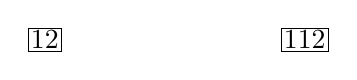
\begin{tikzpicture}
%% \node[draw, inner sep=1pt] (p) at (-3,0) {
%% \specificrover{1}{2}
%% };
%% \node[draw, inner sep=1pt] (p1) at (-0.3,0) {
%% \samerover{1}{2}
%% };
%
\node[draw, inner sep=1pt] (p1) at (-0.3,0) {
\specificrover{1}{2}
};

\node[draw, inner sep=1pt] (p1) at (3,0) {
\dontuseconnection{1}{1}{2}
};
\end{tikzpicture}
}
};
\draw[thick] (-4,2) to (9,2);
\visible<2->{
\node[draw, inner sep=1pt] (p4) at (0.2,0) {
\dontuseconnection{1}{1}{2}
%\specificrover{1}{2}
};
\node[] (depp4p1) at (3.0,0) {\Huge $\Rightarrow$};
\node[draw, inner sep=1pt] (p1) at (5.4,0) {
%\samerover{1}{2}
\specificrover{1}{2}
};
\node[] (not) at (5.4,0) {\includegraphics[scale=0.3]{no.png}};

%\draw[thick, ->] (p4) to (p1);
}
\end{tikzpicture}
}

\end{frame}


\begin{frame}{Transportation Example (NoMystery)}

{\centering

\begin{tabular}{cc}
\begin{minipage}{0.35\textwidth}
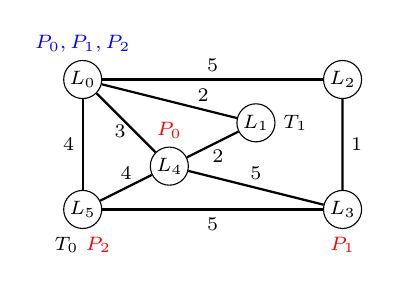
\begin{tikzpicture}[scale=0.55]
	\scriptsize
  \node[draw, circle, inner sep=1pt, label=above:{\textcolor{blue}{$P_0, P_1,P_2$}}] (l0) at (0,0) {$L_0$};
  \node[draw, circle, inner sep=1pt, label=right:{$T_1$}] (l1) at (4,-1) {$L_1$};
  \node[draw, circle, inner sep=1pt] (l2) at (6,0) {$L_2$};
  \node[draw, circle, inner sep=1pt, label=below:{\textcolor{red}{$P_1$}}] (l3) at (6,-3) {$L_3$};
  \node[draw, circle, inner sep=1pt, label=above:{\textcolor{red}{$P_0$}}] (l4) at (2,-2) {$L_4$};
  \node[draw, circle, inner sep=1pt, label=below:{$T_0$ \textcolor{red}{$P_2$}}] (l5) at (0,-3) {$L_5$};

  \draw[thick] (l0) to node[above] {5} (l2);
  \draw[thick] (l0) to node[above, pos=0.75] {2} (l1);
  \draw[thick] (l0) to node[below, pos=0.4] {3} (l4);
  \draw[thick] (l0) to node[left] {4} (l5);
  \draw[thick] (l2) to node[right] {1} (l3);
  \draw[thick] (l4) to node[below, pos=0.6] {2} (l1);
  \draw[thick] (l4) to node[above] {5} (l3);
  \draw[thick] (l5) to node[below] {5} (l3);
  \draw[thick] (l4) to node[above] {4} (l5);
\end{tikzpicture}
\end{minipage} &
\hspace{-0.4cm} \begin{minipage}{0.56\textwidth}
\scriptsize

\begin{itemize}
\item Variables \vars: $T_1, f_1, T_2, f_2, P_0, P_1, P_2$
\item Actions \acts: $drive(T_i,L_x,L_y)$, $load(T_i,P_j,L_x)$, $unload(T_i,P_j,L_x)$

      Driving consumes fuel as indicated
\item Initial state \init: as shown; \textred{$\init(f_1)=16, \init(f_2)=7$}
\item Goal \goalsoft: $at(P_0,L_4), at(P_1,L_3), at(P_2,L_5)$
\end{itemize}

\end{minipage}
\end{tabular}

}

\bigskip \pause

\textbf{Example action-set property analysis:} 

\begin{itemize}
\item 1.\ uses $T_0$ $(L_2,L_3)$; 2.\ same truck 
$P_1$ $P_2$; 3.\ uses $T_0$ $(L_4,L_3)$; 4.\ same truck $P_2$ $P_0$;
5.\ doesn't use $T_0$ $(L_0,L_5)$; 6.\ uses $T_1$ $(L_5,L_4)$.
\item MUGS: \pause 7, each of size 3, including $\{5, 2, 4\}$.
\end{itemize}

\textred{\notesym~User question ``Why do you not avoid the road
$L_0-L_5$ (which has a lot of traffic at the moment)?''} \pause
\textblue{``Because if you don't use that road, then you cannot deliver all
packages with a single truck.''}

\medskip

\end{frame}


\begin{frame}{Experiments: Global Explanations}

\notesym~Blocksworld, NoMystery, Rovers, TPP (top left to bottom right):

\centering

\medskip

\includegraphics[height=0.72\textheight]{plot-actionsetprops-global-coverage}

\smallskip

\end{frame}



%%%%%%%%%%%%%%%%%%%%%%%%%%%%%%%%%%%%%%%%%%%%%%%%%%%%%%%%%%%%%%%%%%%%%%%%%%%%%%%%%
%%%%%%%%%%%%%%%%%%%%%%%%%%%%%%%%%%%%%%%%%%%%%%%%%%%%%%%%%%%%%%%%%%%%%%%%%%%%%%%%%
%%%%%%%%%%%%%%%%%%%%%%%%%%%%%%%%%%%%%%%%%%%%%%%%%%%%%%%%%%%%%%%%%%%%%%%%%%%%%%%%%
%%% NoGood Learning in State Space
%
%%% Timing: XX min

\section[NoGoods]{NoGood Learning in State Space}
\subsection*{}

\begin{frame}{}

\end{frame}



%%%%%%%%%%%%%%%%%%%%%%%%%%%%%%%%%%%%%%%%%%%%%%%%%%%%%%%%%%%%%%%%%%%%%%%%%%%%%%%%%
%%%%%%%%%%%%%%%%%%%%%%%%%%%%%%%%%%%%%%%%%%%%%%%%%%%%%%%%%%%%%%%%%%%%%%%%%%%%%%%%%
%%%%%%%%%%%%%%%%%%%%%%%%%%%%%%%%%%%%%%%%%%%%%%%%%%%%%%%%%%%%%%%%%%%%%%%%%%%%%%%%%
%%% Last Slide & References

\section*{}

\begin{frame}{Last Slide}

{\centering

Thanks for your attention. Questions?

}

\end{frame}

\section*{}

\begin{frame}[allowframebreaks]{References}
\footnotesize
\bibliographystyle{named}
\bibliography{abbreviations,biblio,crossref}
\end{frame}



%%%%%%%%%%%%%%%%%%%%%%%%%%%%%%%%%%%%%%%%%%%%%%%%%%%%%%%%%%%%%%%%%%%
%%%%%%%%%%%%%%%%%%%%%%%%%%%%%%%%%%%%%%%%%%%%%%%%%%%%%%%%%%%%%%%%%%%
%%%%%%%%%%%%%%%%%%%%%%%%%%%%%%%%%%%%%%%%%%%%%%%%%%%%%%%%%%%%%%%%%%%
%%% BACKUP SLIDES


\end{document}
